\documentclass[12pt,twoside]{report}

%%%%%%%%%%%%%%%%%%%%%%%%%%%%%%%%%%%%%%%%%%%%%%%%%%%%%%%%%%%%%%%%%%%%%%%%%%%%%

% Definitions for the title page
% Edit these to provide the correct information
% e.g. \newcommand{\reportauthor}{Timothy Kimber}

\newcommand{\reporttitle}{Analysing property sales data using Machine Learning}
\newcommand{\reportauthor}{Wenxiang Luo}
\newcommand{\supervisor}{Chiraag Lala}
\newcommand{\degreetype}{MSc Computing}

%%%%%%%%%%%%%%%%%%%%%%%%%%%%%%%%%%%%%%%%%%%%%%%%%%%%%%%%%%%%%%%%%%%%%%%%%%%%%

% load some definitions and default packages
%%%%%%%%%%%%%%%%%%%%%%%%%%%%%%%%%%%%%%%%%
% University Assignment Title Page 
% LaTeX Template
% Version 1.0 (27/12/12)
%
% This template has been downloaded from:
% http://www.LaTeXTemplates.com
%
% Original author:
% WikiBooks (http://en.wikibooks.org/wiki/LaTeX/Title_Creation)
%
% License:
% CC BY-NC-SA 3.0 (http://creativecommons.org/licenses/by-nc-sa/3.0/)
% 
%
%%%%%%%%%%%%%%%%%%%%%%%%%%%%%%%%%%%%%%%%%
%----------------------------------------------------------------------------------------
%	PACKAGES AND OTHER DOCUMENT CONFIGURATIONS
%----------------------------------------------------------------------------------------
\usepackage[a4paper,hmargin=2.8cm,vmargin=2.0cm,includeheadfoot]{geometry}
\usepackage{textpos}
\usepackage[numbers]{natbib} % for bibliography
\usepackage{tabularx,longtable,multirow,subfigure,caption}%hangcaption
\usepackage{fncylab} %formatting of labels
\usepackage{fancyhdr} % page layout
\usepackage{url} % URLs
\usepackage[english]{babel}
\usepackage{amsmath}
\usepackage{graphicx}
\usepackage{dsfont}
\usepackage{epstopdf} % automatically replace .eps with .pdf in graphics
\usepackage{backref} % needed for citations
\usepackage{array}
\usepackage{latexsym}
\usepackage[pdftex,pagebackref,hypertexnames=false,colorlinks]{hyperref} % provide links in pdf

\hypersetup{pdftitle={},
  pdfsubject={}, 
  pdfauthor={},
  pdfkeywords={}, 
  pdfstartview=FitH,
  pdfpagemode={UseOutlines},% None, FullScreen, UseOutlines
  bookmarksnumbered=true, bookmarksopen=true, colorlinks,
    citecolor=black,%
    filecolor=black,%
    linkcolor=blue,%
    urlcolor=black}

\usepackage[all]{hypcap}


%\usepackage{color}
%\usepackage[tight,ugly]{units}
%\usepackage{float}
%\usepackage{tcolorbox}
%\usepackage[colorinlistoftodos]{todonotes}
% \usepackage{ntheorem}
% \theoremstyle{break}
% \newtheorem{lemma}{Lemma}
% \newtheorem{theorem}{Theorem}
% \newtheorem{remark}{Remark}
% \newtheorem{definition}{Definition}
% \newtheorem{proof}{Proof}


%%% Default fonts
\renewcommand*{\rmdefault}{bch}
\renewcommand*{\ttdefault}{cmtt}



%%% Default settings (page layout)
\setlength{\parindent}{0em}  % indentation of paragraph

\setlength{\headheight}{14.5pt}
\pagestyle{fancy}
\renewcommand{\chaptermark}[1]{\markboth{\chaptername\ \thechapter.\ #1}{}} 

\fancyfoot[ER,OL]{\sffamily\textbf{\thepage}}%Page no. in the left on odd pages and on right on even pages
\fancyfoot[OC,EC]{\sffamily }
\renewcommand{\headrulewidth}{0.1pt}
\renewcommand{\footrulewidth}{0.1pt}
\captionsetup{margin=10pt,font=small,labelfont=bf}


%--- chapter heading

\def\@makechapterhead#1{%
  \vspace*{10\p@}%
  {\parindent \z@ \raggedright \sffamily
    \interlinepenalty\@M
    \Huge\bfseries \thechapter \space\space #1\par\nobreak
    \vskip 30\p@
  }}

%---chapter heading for \chapter*  
\def\@makeschapterhead#1{%
  \vspace*{10\p@}%
  {\parindent \z@ \raggedright
    \sffamily
    \interlinepenalty\@M
    \Huge \bfseries  #1\par\nobreak
    \vskip 30\p@
  }}

\allowdisplaybreaks

% load some macros
% Here, you can define your own macros. Some examples are given below.

\newcommand{\R}[0]{\mathds{R}} % real numbers
\newcommand{\Z}[0]{\mathds{Z}} % integers
\newcommand{\N}[0]{\mathds{N}} % natural numbers
\newcommand{\C}[0]{\mathds{C}} % complex numbers
\renewcommand{\vec}[1]{{\boldsymbol{{#1}}}} % vector
\newcommand{\mat}[1]{{\boldsymbol{{#1}}}} % matrix


\date{June 2022}

\begin{document}

% load title page
% Last modification: 2015-08-17 (Marc Deisenroth)
\begin{titlepage}

\newcommand{\HRule}{\rule{\linewidth}{0.5mm}} % Defines a new command for the horizontal lines, change thickness here


%----------------------------------------------------------------------------------------
%	LOGO SECTION
%----------------------------------------------------------------------------------------


\includegraphics[width = 4cm]{./figures/imperial}\\[0.5cm] 

\center % Center remainder of the page

%----------------------------------------------------------------------------------------
%	HEADING SECTIONS
%----------------------------------------------------------------------------------------

\textsc{\Large Imperial College London}\\[0.5cm] 
\textsc{\large Department of Computing}\\[0.5cm] 

%----------------------------------------------------------------------------------------
%	TITLE SECTION
%----------------------------------------------------------------------------------------

\HRule \\[0.4cm]
{ \huge \bfseries \reporttitle}\\ % Title of your document
\HRule \\[1.5cm]
 
%----------------------------------------------------------------------------------------
%	AUTHOR SECTION
%----------------------------------------------------------------------------------------

\begin{minipage}{0.4\textwidth}
\begin{flushleft} \large
\emph{Author:}\\
\reportauthor % Your name
\end{flushleft}
\end{minipage}
~
\begin{minipage}{0.4\textwidth}
\begin{flushright} \large
\emph{Supervisor:} \\
\supervisor % Supervisor's Name
\end{flushright}
\end{minipage}\\[4cm]


%----------------------------------------------------------------------------------------
%	FOOTER & DATE SECTION
%----------------------------------------------------------------------------------------
\vfill % Fill the rest of the page with whitespace
Submitted in partial fulfillment of the requirements for the MSc degree in
\degreetype~of Imperial College London\\[0.5cm]

\makeatletter
\@date 
\makeatother


\end{titlepage}



% page numbering etc.
\pagenumbering{roman}
\clearpage{\pagestyle{empty}\cleardoublepage}
\setcounter{page}{1}
\pagestyle{plain}
\graphicspath{ {./figures/} }

%%%%%%%%%%%%%%%%%%%%%%%%%%%%%%%%%%%%
\begin{abstract}
The real estate market is one of the critical aspect of the economy, and the transactions not only affect sellers, buyers and agents, but also it can influence investors and government policies. Therefore, an accurate and non-bias algorithm should be developed to predict if the property transactions can be completed. In this project, the estate information is provided by EweMove and the transaction between 2018 and 2022 are covered. To accurately forecast the transaction status, several artificial neural networks are created initially, then the predicted prices and actual prices, along with the property information are used to train the neural networks for predicting transaction status. To evaluate the performance of models, the mean squared error and coefficient of determination are employed for price predictions. The confusion matrix, accuracy, recall, precision and F1 score are utilized for status predictions, and the model can forecast status with an accuracy of 82.7\%. 
\end{abstract}

\cleardoublepage
%%%%%%%%%%%%%%%%%%%%%%%%%%%%%%%%%%%%
\section*{Acknowledgments}
Comment this out if not needed.

\clearpage{\pagestyle{empty}\cleardoublepage}

%%%%%%%%%%%%%%%%%%%%%%%%%%%%%%%%%%%%
%--- table of contents
\fancyhead[RE,LO]{\sffamily {Table of Contents}}
\tableofcontents 


\clearpage{\pagestyle{empty}\cleardoublepage}
\pagenumbering{arabic}
\setcounter{page}{1}
\fancyhead[LE,RO]{\slshape \rightmark}
\fancyhead[LO,RE]{\slshape \leftmark}

%%%%%%%%%%%%%%%%%%%%%%%%%%%%%%%%%%%%
\chapter{Introduction}

The real estate market is one of the most significant aspects of the economy, and its crisis can influence the entire society, including residents, buyers, sellers, investors, and the governments. Moreover, property prices can be affected by a variety of factors, such as the property layout, local environment, and economic trends. Therefore, reliable predictions generated by a non-bias algorithm are critical in this field. With the help of this algorithm, sellers can obtain reasonable prices for their properties which is advantageous for selling, as the transactions are highly likely to fail if the prices are incredibly high or low. The buyer can benefit from the predictions by avoiding fake information and fraud. Additionally, it will also be profitable for agents since they will be able to find more prospective sellers and buyers, resulting in more successful transactions. 
\\

However, there are extensive data for the real estate market, ranging from different years and all over the world, which can be one of the main obstacles for analysis as it is approximately impossible for humans to obtain insights into the data manually. Under this circumstance, machine learning (ML), a technique that the computer can learn and improve from data without explicit programming, could be one of the methods to mitigate this issue. It can extract patterns from large datasets and use them to make predictions based on the input data and even identify which components are responsible for the results.
\\

In this project, multiple artificial neural networks, one of the ML models, will be constructed to predict property prices initially. The model with the best performance will be selected for subsequent development. Based on this achievement, other neural networks for forecasting if a property can be sold will be created, which is the main objective of this project. 
\\

This report consists of five chapters. In the second chapter, several related papers, such as datasets, models, and applications of ML in real estate, as well as the libraries that will be used in this project, are reviewed. Next, the implementation of this project is described in chapter three. The method for testing and experiment results are demonstrated in the fourth chapter. The last chapter includes a discussion of future work and conclusions. 

%%%%%%%%%%%%%%%%%%%%%%%%%%%%%%%%%%%%
\chapter{Literature Review}
\section{Related Works} 
\subsection{Datasets}
The datasets are the foundation of ML, and a significant number of real estate datasets have been published, some of which are analyzed at the beginning of the project. The first dataset contains the data for Latvia in 2018, which utilizes the real estate announcements posted by one of the most prominent domestic advertisement websites \citep{RN22}. It includes both sale and rental data by region, along with a variety of property types, such as flats, houses, and offices. One of the distinct advantages of this dataset is that the website for updating estate data is monitored by Latvia authorities and is used to enhance the state policy in the real estate market, thereby the reliability of the dataset can be guaranteed.
\\

Nevertheless, the disadvantages of the dataset are noticeable. It only contains the property data in Latvia, suggesting that the conclusions drawn from it might not be applicable to other countries worldwide. Moreover, the regional factors that can significantly influence the real estate transactions, such as economic growth, medical care, and education, are not included in this dataset, meaning that the conclusions base on it only consider the property itself and do not account for the surrounding environment. 
\\

The second dataset contains information on transport, land cover, population density, and real estate for approximately 200 cities worldwide, and 800 million people are covered \citep{RN26}. The dataset utilized GHS-POP and ESA CCI databases for extracting population density and land cover. The real estate, as well as transport information, were obtained via web scrapping and the Google Map and Baidu APIs, respectively.
\\ 

One of the benefits of this dataset is that each city's urban area is divided into 1 km $\times$ 1 km grids, hence the community information, such as distance to the city center and the demographics, can be obtained from this dataset. Moreover, it contains 192 cities around the world, indicating that people from various continents, countries, and cultures are included, allowing for more generalized conclusions to be drawn and making it globally applicable. 
\\

On the other hand, the disadvantage of this dataset is obvious. The interior information of properties is not available, which means that this dataset and the property information should be merged so that ML techniques can be applied. Furthermore, the common limitation of the first two datasets is that they lack records after the outbreak of COVID-19. According to research, the annual loss of the sale and rental prices is 6\%, and the sale prices declined by 13\% one year after the pandemic outbreak \citep{RN29}. Therefore, the accuracy of the models trained by these datasets would be affected. 
\\

The third dataset was employed to evaluate the impact of COVID-19 on the real estate market in Hong Kong (HK). It contains detailed information regarding the infected cases, such as the places patients visited 14 days prior to testing positive. These COVID-19 data are maintained by the HK government, which are updated daily, and the new cases are published within three days after positive testing. The second critical data is the property information that all the patients have been to, including property size, name, and address \citep{RN24}.
\\ 

The distinct advantage of this dataset is that it overcomes the limitation of the first two datasets, which are missing the COVID-19 data. However, its disadvantage is that the dataset is small. The COVID-19 cases between 28 January 2020 and 31 March 2020 were obtained, including 895 cases and 435 corresponding disclosure locations. Therefore, the accuracy of the results of training models with this dataset should be doubted. Moreover, only cases from HK are included in this dataset, meaning that the results can hardly be applied in other areas due to the differences in regional characteristics worldwide. 

\subsection{Models}
\label{model_review}
\subsubsection{K Nearest Neighbor}
K nearest neighbor (KNN) is one of the classification algorithms for supervised learning, which stores all the training data \citep{RN33}. During forecasting, the distances between input and all the training data are calculated, and the prediction would be the class of the training data closest to the input data. The noticeable advantage of this algorithm is that it is simple to implement. In contrast, the disadvantage is obvious; the prediction could be time-consuming due to the computation of the distances to all the training data. 

\subsubsection{Decision Tree}
Decision Tree is another supervised learning algorithm that can be used for classification and regression \citep{RN33}. When training this model,  the data is partitioned into smaller groups recursively based on several metrics, such as information entropy (classification) and variance reduction (regression). One of the benefits of a decision tree is that the outliers cannot significantly influence the performance compared to other algorithms since split conditions generally cause the outliers to be a class by themselves \citep{RN31}. The limitation of the decision tree is that this model is unstable, meaning that its size can be challenging to manage, and changes in the training data may cause substantial modification in the model structure \citep{RN33}. 
\\

There are several variants of the decision tree, one of which is random forest. It consists of multiple decision trees that partition random training data with a random subset of features, resulting in a series of trees capable of producing different predictions \citep{RN34}. Each tree in the forest produces a result when forecasting, and the majority of the predictions are considered the correct result. Another variant is gradient boosting, which is comprised of multiple decision trees. Unlike random forest, a loss function is determined before training. Then the base predictors, i.e., decision trees, are trained with selected metrics to ensure performance. Next, the tree is inserted into the forest if the overall performance can be enhanced \citep{RN35}. 

\subsubsection{Neural Network}
The neural network is a typical algorithm for ML which simulates the principle of biological neural networks and consists of three fundamental concepts, including artificial neurons, network architecture, and learning \citep{RN36}. Similar to biological neurons, artificial neurons determine how to process data based on the inputs and their weights. The architecture of neural networks varies on the number of layers and neurons in each layer. The network is learning by updating its weights to minimize the loss when training data are provided. The remarkable advantage of applying neural networks is that they can extract patterns and insights from a vast amount of data, which is impossible to handle manually. In contrast, the limitation of the neural network is that it generally contains a significant number of parameters that are updated during training which is time-consuming. 

\subsection{Machine Learning Approaches}
In a similar study to this project, \citet{RN17} devised a reliable method for predicting the prices in Riyadh, Saudi Arabia. The attributes of properties, such as location, area, type, and price, are identical to the dataset in this project. However, the interior layouts and facilities, such as parking spaces, outside areas, and heating, were not covered in their study; hence their dataset was inferior to the one in this project. Furthermore, their study was based on the properties in a Middle East country, which is significantly different from the UK in all aspects, such as culture and climate, indicating that the results were unlikely to be applicable to the current project. Various models were utilized, including decision tree, random forest, and linear regression. As a result, the random forest has the best performance among the three algorithms. However, the accuracy in percentage cannot be obtained since they utilized mean absolute error, mean squared error, and median squared error for evaluation. Future improvements include incorporating more data in Riyadh and considering economic trends as a factor that can influence the prices. In addition, other ML models are also encouraged in order to improve performance. 
\\

In another research, \citet{RN20} developed a ML model for forecasting property prices. The dataset they used is maintained by the Florida authority, and the transactions between 2010 and 2019 were collected, comprising approximately 100000 records. Additionally, the economic trends, such as gross domestic product (GDP) and custom price index (CPI), were obtained and incorporated into the property transactions \cite{RN20}. Their dataset is superior to that of the current project since it contains more records and considers the local economics. A variety of ML algorithms, including logistic regression, random forest, voting classifier, and XGBoost were employed to solve the problem accurately. Consequently, they stated that the XGBoost offers the best performance with 92\% and 93\% accuracy when economics are excluded and included, respectively. The results of their study can be referred to in the current project since they used data from the US, which shares some similarities with the UK.
\\

\citet{RN37} analyzed the impact of environmental quality on estate prices in Italy by employing artificial neural networks. A geographic information system provided the property information utilized in their study, and the regional agency in Italy offered the environmental data, resulting in a dataset containing fewer than 200 records. As a result, they concluded that the correlation coefficient (R-value) is approximately 0.895, indicating the coefficient of determination ($R^2$) is 0.81. Moreover, they evaluated which input variable had the most significant influence on the estate price. In order to achieve this objective, they trained the model multiple times, and one of the inputs was excluded each time. R values were used to analyze the effect, meaning that the removal of the significant variable causes the decrease in R-value. Their study's accuracy may be questioned due to the small dataset. However, the methodology can be applied to the current project since applying a neural network does not require extracting features manually. In addition, the method for identifying the variable with the most significant impact on the output can be implemented in this project.

\section{Related Tools}
Python is one of the most popular programming languages in the world since it is simple to develop, and there are extensive packages for various functionalities. In this project, Python and its packages would be used for loading data, preprocessing data, and constructing and evaluating ML models. 

%\begin{enumerate}
	%\item Data Preprocessing: Some data from the dataset may be missing, and these values must be handled appropriately before being passed to the model. 
	%\item Standardization: In real life, different features usually have different ranges, and this will cause a problem in ML, which is that high magnitude features would have more weight than low magnitude features \citep{RN4}. One of the solutions is standardization, which could scale all the features to the same magnitude.
	%\item Feature encoding: ML models require numerical values, whereas the categorical features in the dataset do not satisfy this requirement. Therefore, these features should be converted into numerical values. 
	%\item Training \& Testing: The parameters of the model are updated, and it is expected that the loss will converge during training. The performance of the model is validated when testing.
%\end{enumerate}

\subsection{Handle Text Information}
The format of texts in this project could be classified as HTML and plaintext. Although Python standard libraries provide some string processing capabilities, they are insufficient for this situation. 

\subsubsection{Beautiful Soup}
\textit{\textbf{Beautiful Soup}} is a Python library for extracting data from markup languages, such as HTML and XML. It can accomplish this with a user-specified parser, for example, \textbf{\textit{html.parser}}, to navigate, search and modify the parse tree, which would save considerable time \citep{RN10}. 

\subsubsection{parse}
The \textit{\textbf{format}} function in the Python standard library formats a string, whereas the \textit{\textbf{parse}} module provides functions with an oppositse effect, i.e., extract information from formatted strings.

\subsubsection{Regular Expression}
A regular expression is a sequence of ordinary and special characters representing textual patterns. The ordinary characters are identical throughout the expressions and texts, while the special characters specify the pattern, including number, location, and type of characters  \citep{RN14}. One of the primary disadvantages of the regular expression is its obscure syntax, which results in difficulty specifying a pattern. 

\subsubsection{Library Usage}
In this project, HTML texts are used extensively in the raw dataset to describe property summaries, property layouts, and council tax. This is the optimal scenario for \textit{Beautiful Soup} which is employed to extract plaintext by specifying tags. Then, \textit{parse} is applied to obtain the information, such as room names, from the plaintexts since they are in the same format. In addition, due to its limitations, the regular expression is only used to acquire numerical values in this project. 


\subsection{Data Manipulation}
\subsubsection{NumPy}
Numerical Python (\textit{\textbf{NumPy}}) is a scientific computing package designed to support large multidimensional matrices. It uses an optimized \textit{C/C++} API to reduce computation time compared to pure Python computations \citep{RN6}. A substantial number of complex tasks of data analytics can be simplified by numerous \textit{numpy} features. For example, it provides robust matrix operations, facilitates the construction of multidimensional objects, and serves as the foundation of other packages, including \textit{matplotlib} and \textit{seaborn}.

\subsubsection{Pandas}
The \textbf{\textit{pandas}} is an open-source and compelling package that was developed primarily for data analysis and data manipulation and is built on \textit{numpy}. It is capable of handling data of various types (numerical values, strings, and time) and from a variety of sources (CSV, Excel, and MqSQL database). \textbf{\textit{DataFrame}} is one of the \textit{pandas} data structures that is appropriate for handling tabular data with columns of different types. Additionally, it could manage various operations, such as manipulating missing values, creating pivot tables, and grouping data from different columns \citep{RN4}. 

\subsubsection{Library Usage}
In this project, the dataset provided is in CSV format hence it could be loaded by \textbf{\textit{Pandas}} since it is suitable for tabular data. Then the package is utilized for preprocessing, such as handling missing values and grouping columns of data. 
\\

\textit{\textbf{Numpy}} is appropriate for manipulating numerical data and acts as an intermediary between various packages. Therefore, it could be employed to evaluate the performance of ML models and transmit data to plotting packages. 


\subsection{ML Frameworks}
\subsubsection{Scikit-learn}
\textit{\textbf{Scikit-learn}} is a popular open-source ML framework that employs \textit{Numpy}. It contains traditional ML algorithms, including clustering, classification, and regression, as well as a variety of utilities that can be applied to preprocess data and evaluate the performance \citep{RN7}. The drawback of this library is that it does not natively support GPU acceleration and is not a neural network framework. 

\subsubsection{PyTorch}
\textbf{\textit{PyTorch}} is one of the popular ML frameworks developed by Facebook, which is designed to implement neural networks with flexibility and speed \citep{RN5}. It provides various components for model construction and training. For instance, there are numerous types of modules that comprise a model, such as linear layers, dropout, and activation functions, as well as a variety of loss functions and optimizers that can be employed in model training. 
\\

Furthermore, it can be beneficial to construct and train a model with \textit{Pytorch}. It has a Pythonic nature which means that its syntax is similar to Python, making it more straightforward for Python programmers to develop neural networks than other ML frameworks. Moreover, it is a rapidly expanding framework for developing neural networks with a vast ecosystem, meaning that a substantial number of utilities have been developed on top of it \citep{RN5}. Additionally, \textit{PyTorch} supports automatic differentiation and GPU acceleration which can be advantageous for model training.

\subsubsection{TensorFlow}
\textit{\textbf{TensorFlow}} is another ML framework produced by Google that specializes in deep learning and neural networks. It provides approximately the same components as \textit{PyTorch} and also supports automatic differentiation and GPU acceleration. One of the appealing characteristics of \textit{TensorFlow} is called \textit{\textbf{TensorBoard}}, which is an interactive visualization system that can display the flowchart of the data manipulation and plot the tendency of the performance \citep{RN15}. 

\subsubsection{Library Usage}
This project aims to construct a neural network which means \textit{scikit-learn} is not applicable at this stage. Although \textit{TensorFlow} provides the same capabilities as \textit{PyTorch} and is superior in visualization, the model construction and training will use \textit{PyTorch} due to its Pythonic syntax and compatibility with \textit{TensorBoard}. 
\\

However, \textit{scikit-learn} can be used to preprocess datasets and evaluate performance. It provides various utilities that can be helpful before training, for example, encoding categorical features and splitting the dataset into training and validation. In addition, it offers features for model evaluation, such as confusion matrix, accuracy, and recall. 

\subsection{Data Visualization}
\subsubsection{Matplotlib}
\textbf{\textit{Matplotlib}} is a Python package for 2D plotting that produces high-quality figures. It supports interactive and non-interactive plotting and can save images in multiple formats, including PNG and JPEG. It can also generate numerous types of graphs, such as line plots, scatter plots, and pie plots.

\subsubsection{Seaborn}
\textbf{\textit{Seaborn}} is a Python library for creating statistical graphs that integrates with \textit{pandas} to offer a high-level interface to \textit{matploblib}. If a dataset is provided, \textit{seaborn} can automatically generate the figure with appropriate plotting attributes, such as color and legend. Additionally, it is capable of generating comprehensive graphics with a single function call and a minimum number of arguments \citep{RN16}.

\subsubsection{Library Usage}
In this project, data visualization would be beneficial during preprocessing data and performance evaluation. For preprocessing, the distribution of the raw data should be inspected, hence \textit{seaborn} could be an optimal choice since the input is a \textit{DataFrame} and its syntax is concise. During evaluation, the model output will be converted to \textit{Numpy} arrays. Therefore, \textit{matplotlib} can be used in this case, as it is interactive and the figure can be further adjusted to illustrate the performance. 

\section{Research Gap}
Most of the research focused on predicting the prices for real estate, and various ML algorithms were employed. However, there are insufficient studies on forecasting whether the property transaction can be completed. Therefore, this project develops artificial neural networks for predicting the status of transactions in the real estate market, and the property layout and facilitates are considered. 

%%%%%%%%%%%%%%%%%%%%%%%%%%%%%%%%%%%%%%%%%%%%%%%%%%%%%%%%%%%%%%
\chapter{Implementation}

\section{Methodology}
\subsubsection{Data Preparation}
The raw data should be preprocessed, and the steps are as follows. 
\begin{enumerate}
	\item Handling missing values: They must be handled appropriately before being passed to the model. The possible methods include removing missing values and replacing them with the default value.
	\item Standardization: In real life, different features usually have different ranges, which will cause a problem in ML, which is that high magnitude features would have more weight than low magnitude features \citep{RN4}. One of the solutions is standardization, which could scale all the features to the same magnitude.
	\item Feature encoding: ML models require numerical values, whereas the categorical features in the dataset do not satisfy this requirement. Therefore, these features should be converted into numerical values.
\end{enumerate}

The datasets created during preprocessing are split into training and testing sets, representing 90\% and 10\% of the total dataset, respectively. In the meantime, the datasets are also shuffled as they may contain intrinsic patterns.

\subsubsection{Training models}
Due to the limited training data for this project, cross validation is employed to train the model with different portions of training data. There are two model outputs, including prices and the status of transactions. The loss function for prices is mean squared error (MSE) as they are positive values. However, the status of transactions is either one or zero, hence its loss function is binary cross entropy (BCE). 
\\

The optimizer used for training is Adam, which could compute a learning rate for each parameter and has a low computing time. The learning rate is initially set to $1 \times 10^{-3}$ and would be updated if necessary.
\\

The performance is illustrated after cross validation by plotting training and validation losses against epoch. Based on these graphs, the model with the best performance can be selected for the evaluation phase. 

\subsubsection{Evaluation}
The model performance should be evaluated on unseen data. Otherwise, it would be useless. Various metrics are used to quantify the performance of the model in this project. 
\\

As the measurements for predicted prices, MSE, and coefficient of determination ($R^2$) are applied.  The lower the MSE, the better the performance. $R^2$ values are typically between 0 to 1. A model with $R^2 = 0$ means the model cannot make accurate predictions, while $R^2 = 1$ indicates that the model can precisely predict the results. In rare instances, the $R^2$ can be negative, indicating that the model does not match the trend of the data, which is the worst performance. 
\\

The confusion matrix is initially obtained to access the predictions regarding the status of transactions. A confusion matrix summarizes the classification results, indicating where the model outputs wrong predictions and the types of errors. Based on the confusion matrix, various metrics are calculated, and they are shown as follows, 
\begin{itemize}
	\item \textbf{Accuracy}: It is the number of correct predictions divided by the total number of predictions. The best accuracy is one and zero is the worst. 
	\item \textbf{Precision}: It is the number of correct positive predictions divided by the total number of positive predictions. High precision suggests that predictions on positive can be guaranteed.
	\item \textbf{Recall}: The ratio of correct positive predictions to the total number of positive examples, and the high recall indicates that the positive class is correctly identified. 
	\item \textbf{F1 Score}: This is a harmonic mean of both recall and precision which can be used to evaluate performance independently. 
\end{itemize}

\section{Data Source and Collection}
The datasets used in this project are provided by EweMove, and transactions from 2018 to 2022 are included. There are 34591 records with 36 parameters describing each property after merging these datasets. Some parameters, such as postcodes, and room information, are independent variables that would be the model input. In contrast, the price and status of the transaction are dependent variables that serve as labels of supervised learning. The features that are used in this project are listed in table \ref{model_input_features}. 

\begin{table}[H]
	\centering
	\caption{The features used to train the model}
	\label{model_input_features}
	\begin{tabular}{| l | l | l |}
		\hline
		\textbf{Feature} & \textbf{Description} & \textbf{Type} \\
		\hline
		Postcode & / & Categorical \\
		\hline
		Sale or Let & / & Categorical \\
		\hline
		Description S3 Rooms & The room names and dimensions & HTML texts\\
		\hline
		RTD3308\_outside\_space & Keywords describing outside spaces & Categorical \\ 
		\hline
		RTD3307\_parking& Keywords describing parking & Categorical \\
		\hline
		RTD3316\_condition & The condition of the property & Categorical \\
		\hline
		RTD3318\_heating & Keywords describing heating & Categorical \\
		\hline
		RTD3317\_accessibility & Keywords describing accessibility & Categorical \\
		\hline
		Price / Rent & / & HTML texts \\
		\hline
		Price Qualifier & The seller can choose how to qualify the price & Categorical \\
		\hline
		DESC Council Tax Band & / & Categorical \\
		\hline
		\# of Enquiry or viewings & / & Numerical \\
		\hline
		\# of Apps/Offers & / & Numerical \\
		\hline
	\end{tabular}
\end{table}

\section{Data Preprocessing}

\subsection{Handle Room Descriptions (HTML)}
\subsubsection{Acquire room name and dimension}
The structure of the HTML texts containing the room information in a property is shown in figure \ref{html_structure}. The rooms are separated by tag \textit{$<$li$>$}, and the room name and its dimension are denoted by \textit{$<$strong$>$} and \textit{$<$i$>$} tags, respectively. Therefore, a function (\textit{\textbf{EweMove\_Description\_S3\_Rooms}}) is implemented to split the HTML texts by utilizing \textit{Beautiful soup}, and its flowchart is shown in figure \ref{html_room_info}.
\begin{figure}[H]
	\centering
	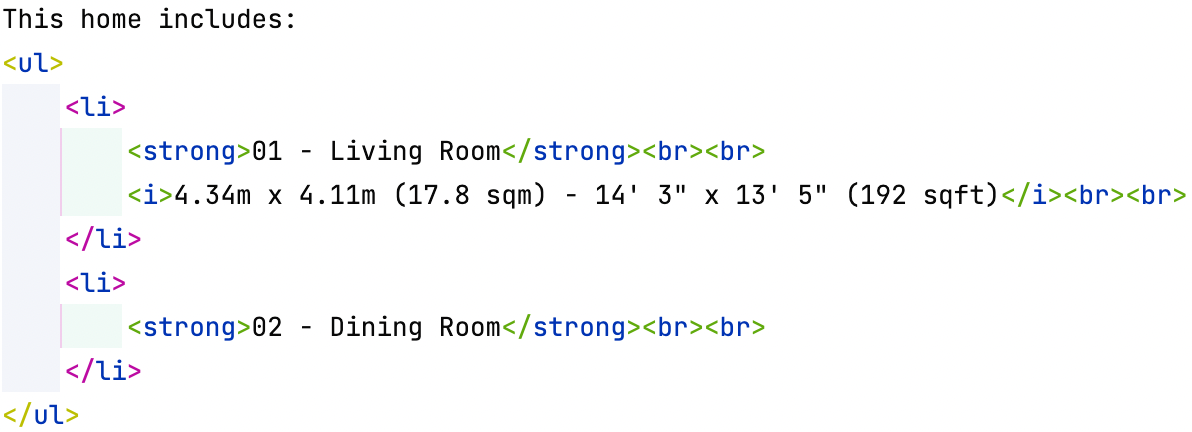
\includegraphics[width=15cm]{html_structure}
	\caption{The layout of HTML texts}
	\label{html_structure}
\end{figure}

\begin{figure}[!htbp]
	\centering
	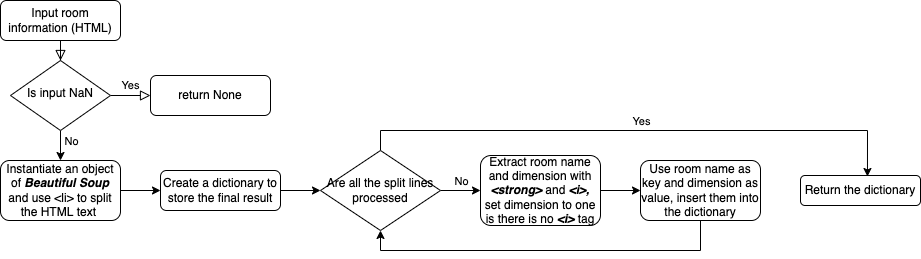
\includegraphics[width=1\linewidth]{html_room_info}
	\caption{Flowchart for extracting room information from HTML}
	\label{html_room_info}
\end{figure}

The names of rooms are analyzed after the room descriptions in the dataset have been processed. As a consequence, there are over 200 unique room names for approximately 36000 records, some of which are exceptionally uncommon across the entire dataset. For instance, only two properties have cinema rooms, and one has a lift, which is less than 0.1\% of all entries.  
\\

Due to the large number of room names, it is impossible to use it as the input of the model. Therefore, the rooms are divided into six categories: bedrooms, bathrooms, kitchens, living/reception rooms, dining rooms, and other rooms so that the data can be generalized. 
\\

\subsubsection{Generalize room information}
A class, \textit{\textbf{ExtractRooms}}, is developed to acquire and integrate the room information, especially the area in square meters, and its UML diagram is shown in figure \ref{uml_extract_rooms}. The member variable \textit{rooms} is a list containing the result of invoking \textit{EweMove\_Description\_S3\_Rooms}, \textit{room\_set} comprises all the room names, \textit{current\_rooms} consists of the room names that have been processed, and \textit{extract\_area} is a formatted string for acquiring room area. 
\\

\begin{figure}[!htbp]
	\centering
	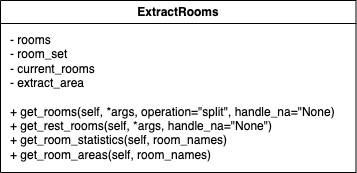
\includegraphics[width=10cm]{uml_extract_rooms}
	\caption{The UML diagram of the class (\textit{ExtractRooms})}
	\label{uml_extract_rooms}
\end{figure}

There are two essential member functions, the first one is \textit{\textbf{get\_rooms}}, and its flow diagram is shown in figure \ref{extract_room_get_rooms} and the arguments are listed below. 
\begin{enumerate}
	\item args: It should be noted that this is a variable-length argument, which means that it can accept as many arguments as possible, and it is used to select room names from \textit{room\_set}. For instance, \textit{*args = [living, reception]} will select all names containing \textit{living} or \textit{reception}. 
	\item operation: The argument determines the types of the final result and the valid inputs include \textit{sum}, \textit{mean}, \textit{split}, and \textit{number}. For example, if args is \textit{bedroom}, then the function can return the sum of bedroom areas, the average bedroom area, the area of each bedroom and the number of bedrooms. 
	\item handle\_na: This parameter specifies how to manage missing values, either by ignoring them or by filling the mean value if the input is \textit{None} or \textit{mean}, respectively. 
\end{enumerate} 

\begin{figure}[!htbp]
	\centering
	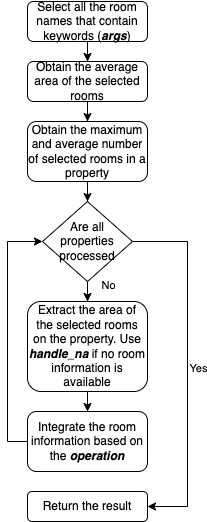
\includegraphics[width=\linewidth]{extract_room_get_rooms}
	\caption{Flowchart of \textit{get\_rooms}}
	\label{extract_room_get_rooms}
\end{figure}

The second member function is \textit{\textbf{get\_rest\_room}}. It is identical to \textit{get\_room} with two exceptions. The parameter \textit{\textbf{*args}} is used to disgard the room names containing the keywords, and only the number and the total areas of other rooms are returned. 

\subsection{Manipulate Categorical Keywords}
In the dataset, four features are characterized by categorical keywords, including parking, heating, accessibility, and outdoor spaces. Figure \ref{parking_dataset} is a snippet of the parking dataset that is used as an example to illustrate the manipulation of the keywords. The first three rows indicate that there is a parking space for the first property, which is \textbf{allocated} \textbf{off-street} parking for \textbf{residents}, the second has none, and the third property has one \textbf{on-street} parking space. This principle applies to other rows as well. In this situation, feature encoding cannot be applied since there are multiple columns of keywords describing a feature, and the order and quantity of the keywords have no effect.
\\

\begin{figure}[!htbp]
	\centering
	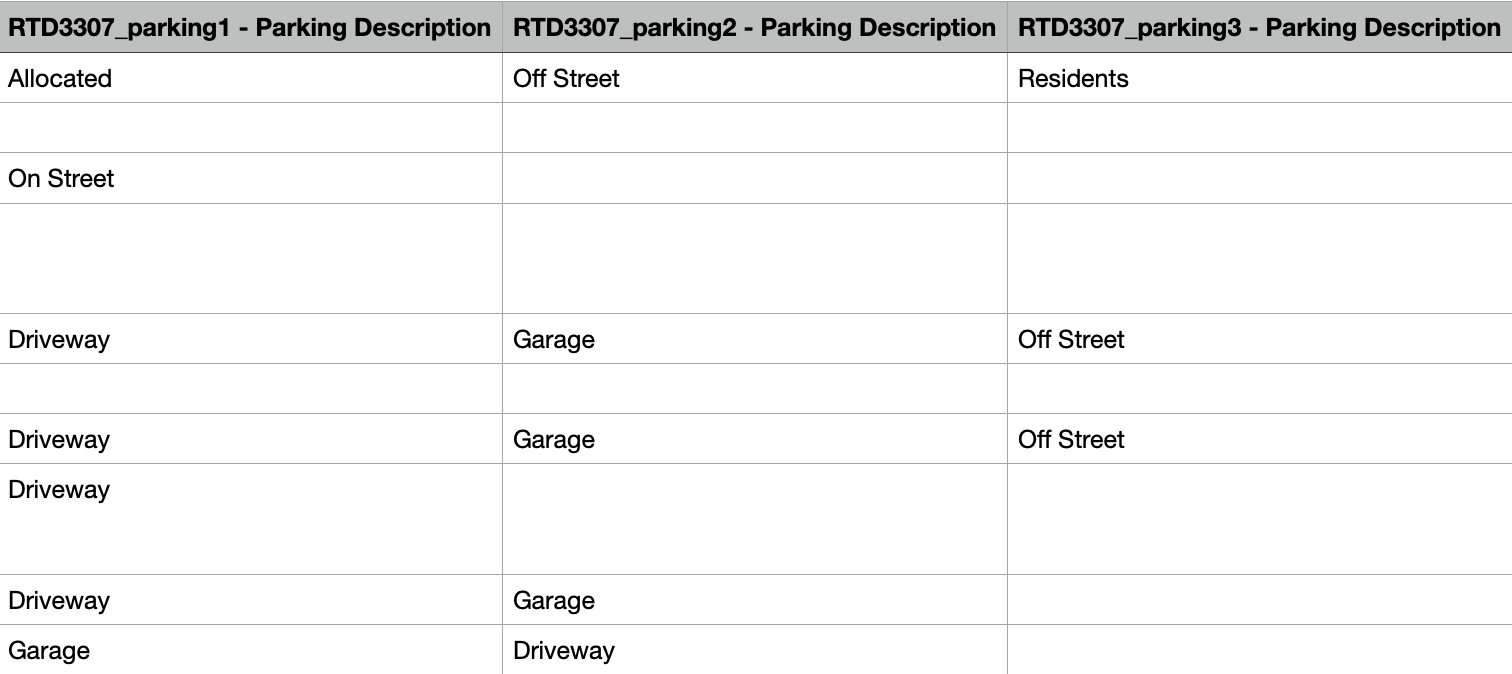
\includegraphics[width=12cm]{parking_dataset}
	\caption{The parking spaces in the first five properties}
	\label{parking_dataset}
\end{figure}

Figure \ref{uml_generalize_dataset} illustrates the UML diagram of the class \textit{\textbf{GeneralizeDataset}}, which is developed to determine how these features of each property are described and the number of keywords within the description. The core of this class is member function \textit{\textbf{get\_feature\_types}}, and its flowchart is displayed in figure \ref{generalize_dataset_get_feature_types}. In addition, function \textbf{\textit{get\_feature\_num}} can be used to determine the number of keywords for each property. 
\\

\begin{figure}[!htbp]
	\centering
	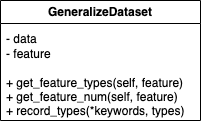
\includegraphics[width=6cm]{uml_generalize_dataset}
	\caption{The UML diagram of \textit{GeneralizeDataset}}
	\label{uml_generalize_dataset}
\end{figure}

\begin{figure}[!htbp]
	\centering
	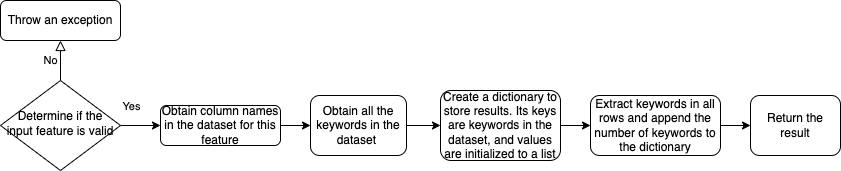
\includegraphics[width=1\linewidth]{generalize_dataset_get_feature_types}
	\caption{Flowchart of \textit{get\_feature\_types}}
	\label{generalize_dataset_get_feature_types}
\end{figure}

\subsection{Manage Outliers}
The price is crucial to the project, and the distribution of the raw data is inspected, as shown in figure \ref{price_raw}. The spike on the left side of the figure indicates that numerous properties have zero prices, which is illogical. Therefore, these abnormal values should be addressed as they could significantly impact the performance of the model.

\begin{figure*}[!htbp]
	\centering
	\subfigure[All Prices]{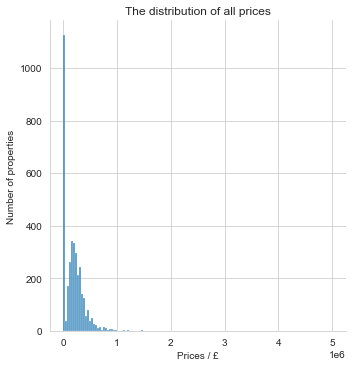
\includegraphics[width=5cm]{price_all_raw}\label{price_all_raw}}
	\hfill
	\subfigure[Sale Prices]{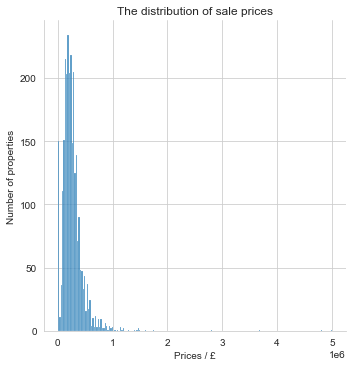
\includegraphics[width=5cm]{price_sale_raw}\label{price_sale_raw}}
	\hfill
	\subfigure[Rental Prices]{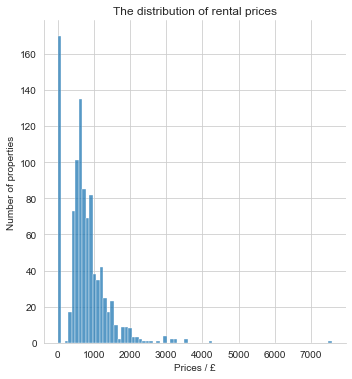
\includegraphics[width=5cm]{price_rental_raw}\label{price_rental_raw}}
	\caption{The distribution of prices from raw data}
	\label{price_raw}
\end{figure*}

\subsection{Create Input Dataset}
\label{create_input_dataset_section}
\subsubsection{Feature Encoding}
This technique is applicable to categorical features in the dataset, including price qualifier, council tax band, and property condition. The label encoding is employed, which is capable of converting the feature into numeric values between 0 and N - 1, where N is the number of distinct classes in a column.

\subsubsection{Manage Missing Values}
The datasets used in this project contain a significant number of missing values. For example, approximately 30\% of the room layout and more than 40\% of the council tax band are missing. Under this situation, it is impossible to replace them with the mean value since it causes the model to focus on the average and result in low performance. Therefore, another approach is applied, which is removing the missing values in the datasets. 

\subsubsection{Classy Approach}
After the information in HTML texts and categorical keywords are extracted, it is combined with other columns in the dataset to produce a clean dataset for the model input.  Figure \ref{uml_create_input_dataset} is the UML diagram of \textit{\textbf{CreateInputDataset}}, which is a class developed for this objective, and the flow diagram of producing an input dataset is displayed in figure \ref{create_input_dataset}.

\begin{figure}[!htbp]
	\centering
	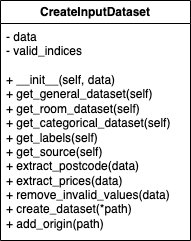
\includegraphics[height=6cm]{uml_create_input_dataset}
	\caption{The UML diagram of \textit{CreateInputDataset}}
	\label{uml_create_input_dataset}
\end{figure}

\begin{figure}[!htbp]
	\centering
	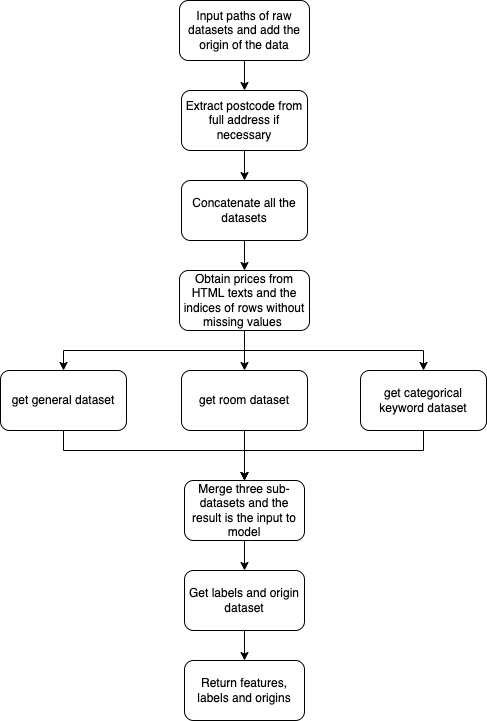
\includegraphics[height=10cm]{create_input_dataset}
	\caption{The flow diagram of producing  input dataset}
	\label{create_input_dataset}
\end{figure}

\section{Model Construction}

\subsection{Basic Model: Output Sale Status and Price}
\label{basic_model_price_status_construction}
The architecture of this model solely consists of linear layers and activation functions, as depicted in figure \ref{basic_model_layout}. There are two outputs of the model, which are prices and the status of transactions. Therefore, the activation functions of the output layers are ReLU and sigmoid, respectively.
\\

\begin{figure}[!htbp]
	\centering
	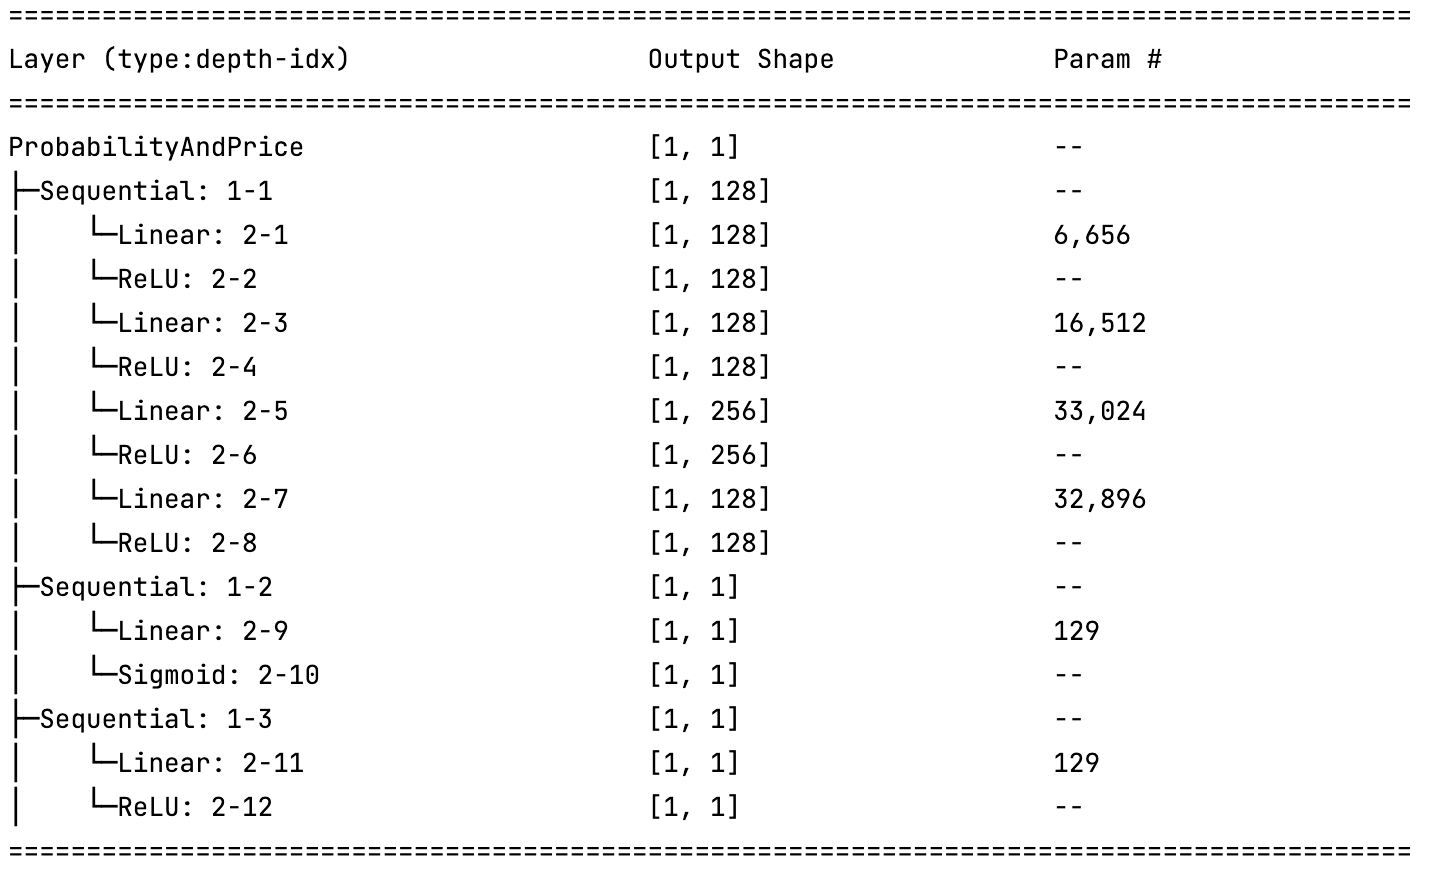
\includegraphics[height=12cm]{basic_model_layout}
	\caption{The architecture of the basic model}
	\label{basic_model_layout}
\end{figure}

\subsection{Linear Regression: Predict Price}
\label{linear_regression_model_construction}
Prior to the construction of any neural networks for predicting prices, a linear regression model with a single linear layer is developed. Its input size is the same as the number of features, and the output is the price. If this model can accurately predict the price, it eliminates the need to build more complex neural networks with multiple layers, which is the motivation for its creation. 

\subsection{Basic Model: Predicting Prices}
The structure of this model is demonstrated in figure \ref{basic_model_price}. Its hidden layers are identical to the model for predicting status and prices (section \ref{basic_model_price_status_construction}), whereas the status output is removed.

\begin{figure}[h]
	\centering
	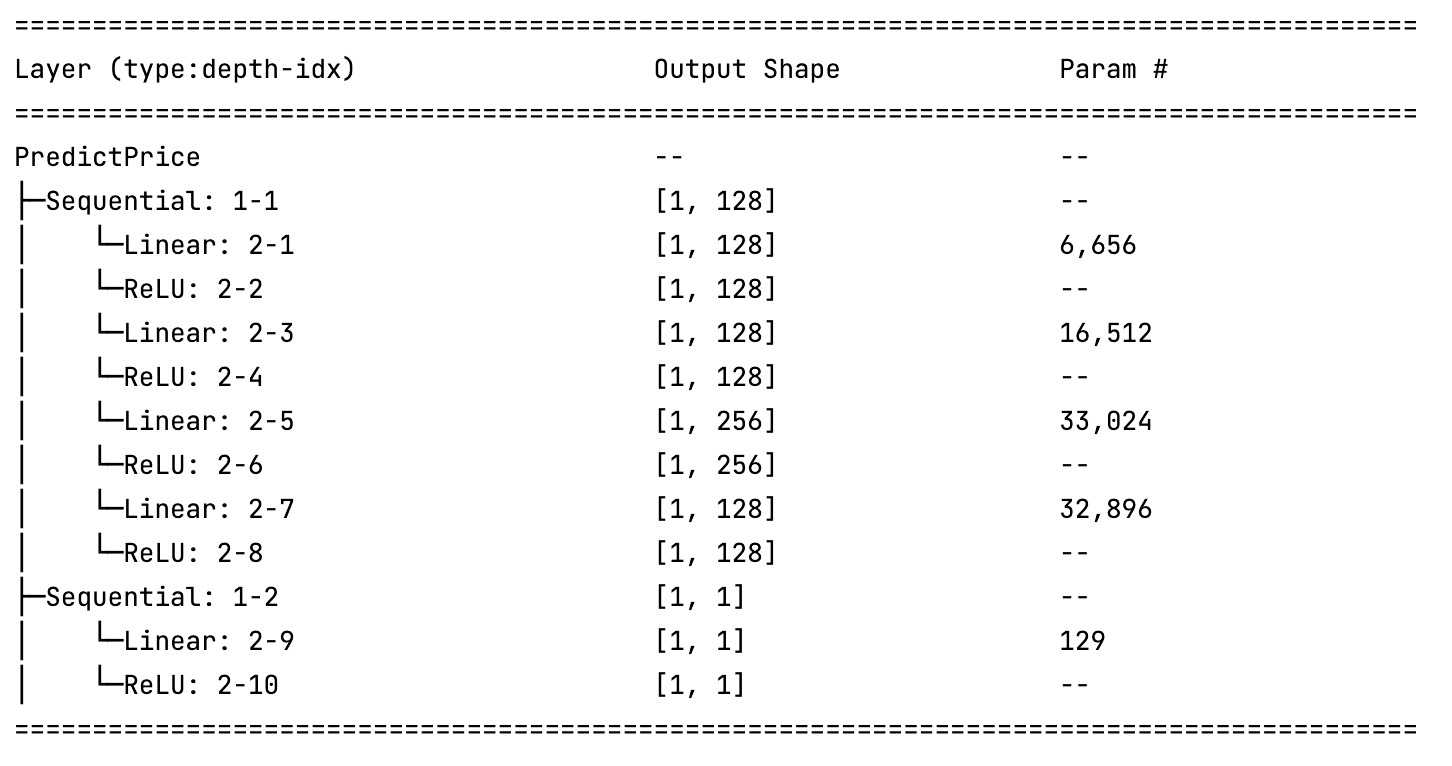
\includegraphics[height=13cm]{basic_model_price}
	\caption{The structure of the basic model for predicting prices}
	\label{basic_model_price}
\end{figure}

\subsection{Complex Model: Predicting Prices}
\label{complex_model_construct}
The layout of a more complex model is similar to that of figure \ref{basic_model_price}, but it contains ten linear layers and there are 512 neurons in each layer. The model is constructed for an obvious reason. Intuitively, more complex models are more capable to learn from the input dataset, resulting in enhanced performance. 

\subsection{Residual Network: Predicting Prices}
The second complex model is developed which utilized residual connections. The architecture of the residual blocks and the network are illustrated in figure \ref{resnet}. This model is developed because the performance of the first complex model (section \ref{complex_model_construct}) is not significantly enhanced despite having more layers and neurons. In addition, tuning the hyperparameters is time consuming and the improvement of the accuracy is limited. 

\begin{figure*}[!htbp]
	\centering
	\subfigure[Residual Block]{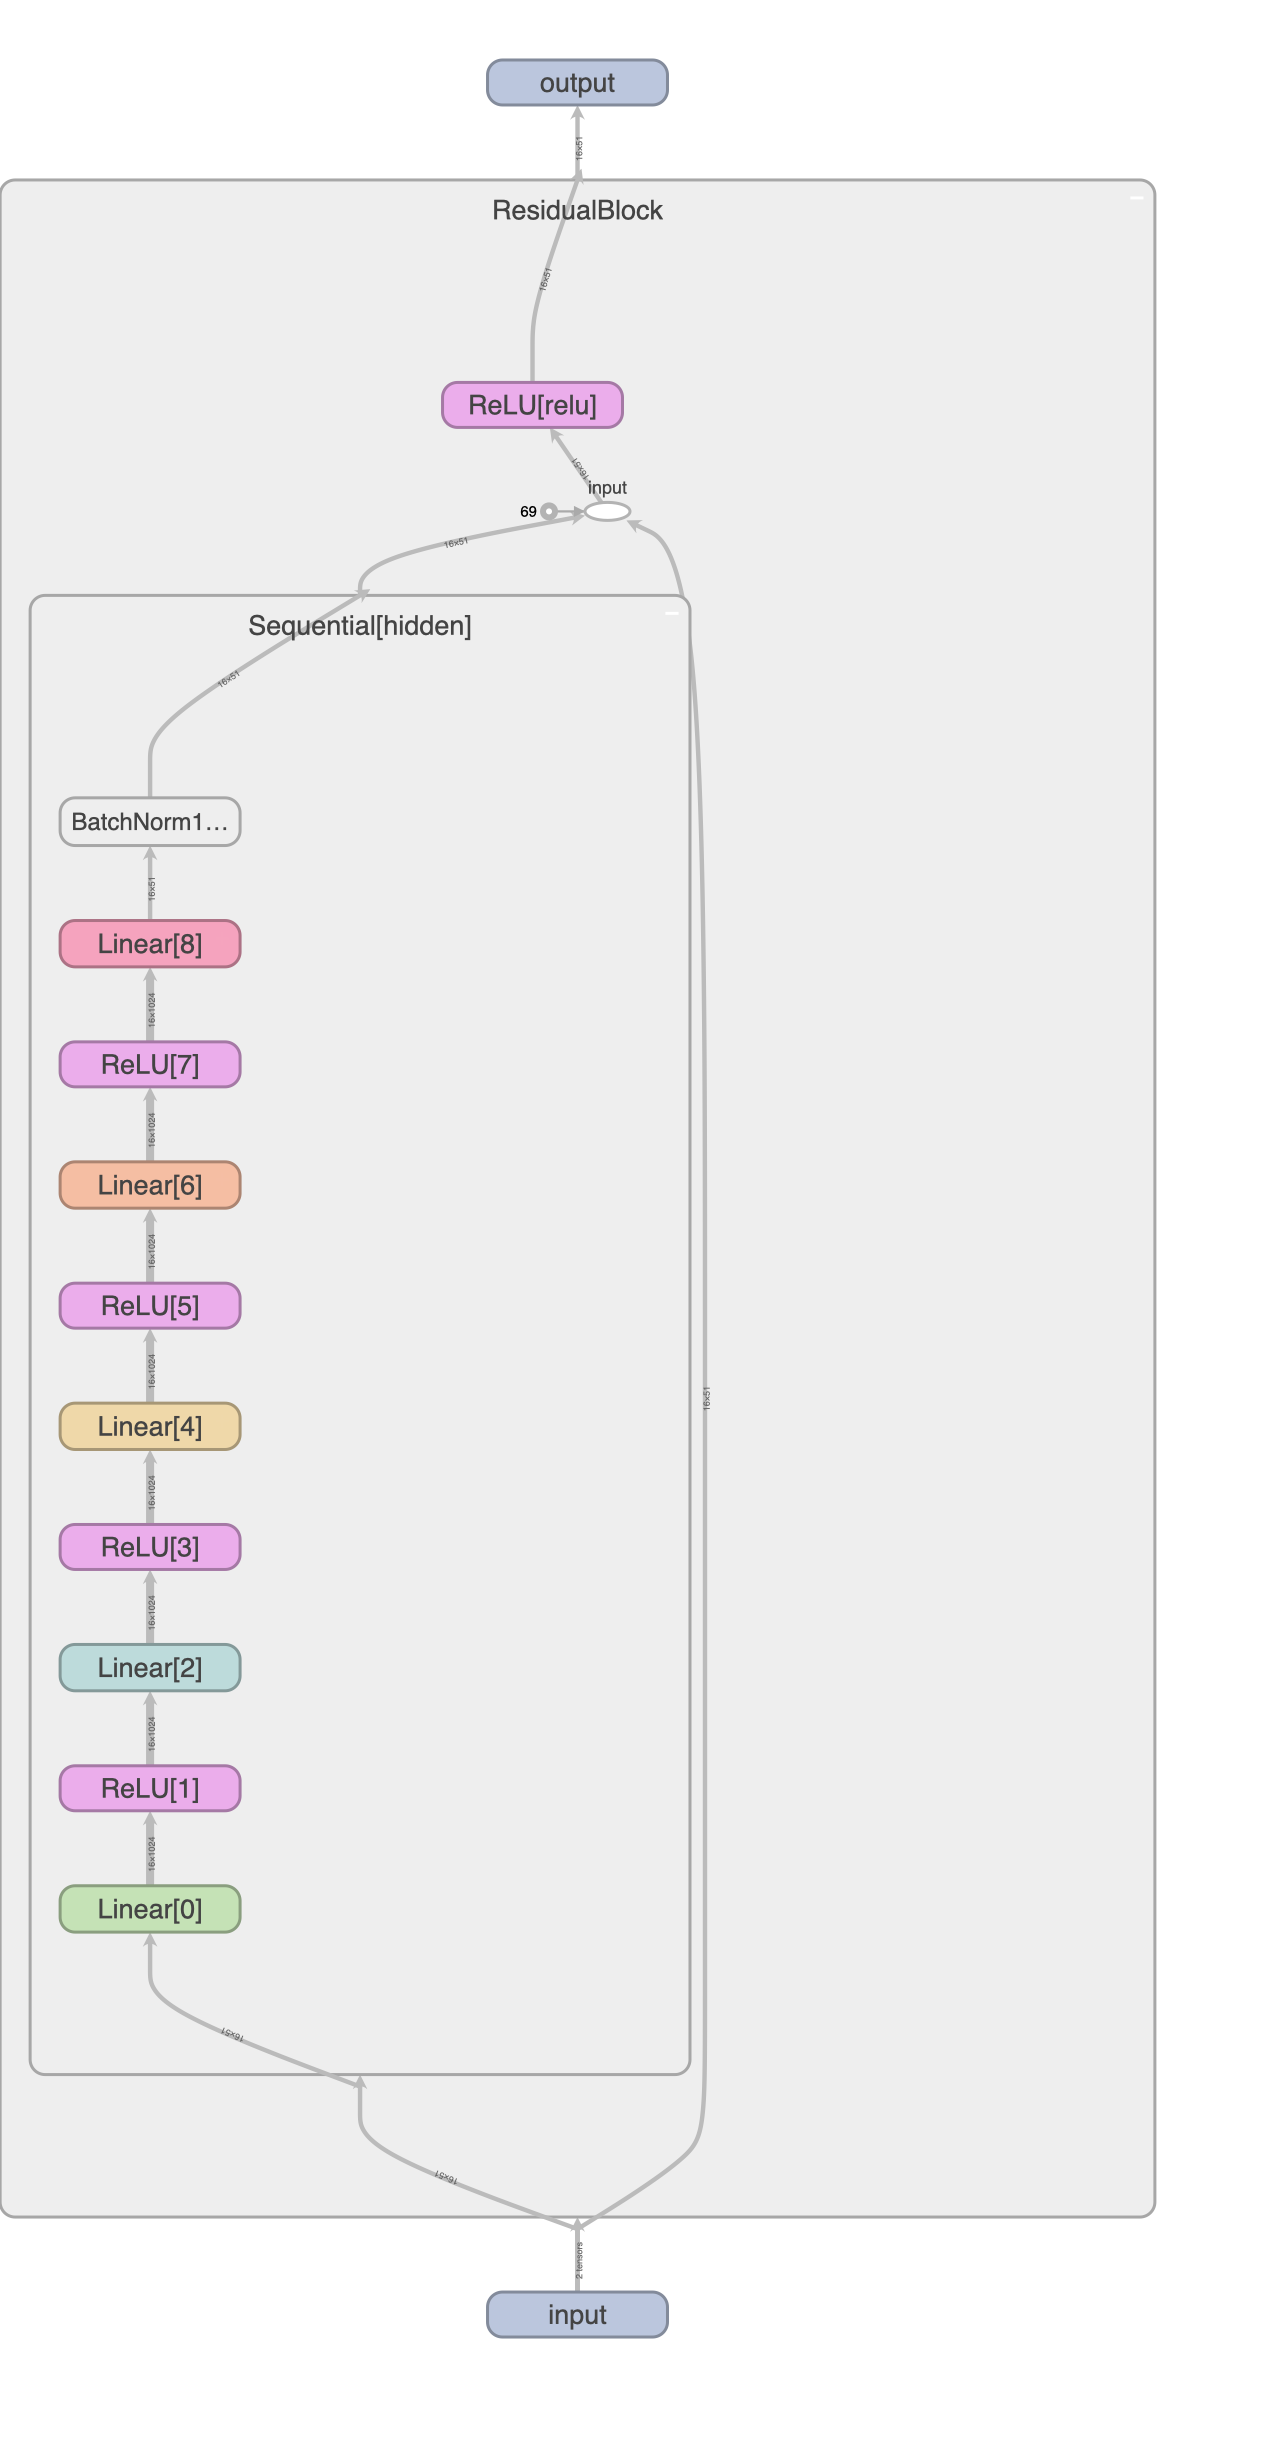
\includegraphics[width=7.5cm]{residual_bolck_layout}}
	\hfill
	\subfigure[Residual Network]{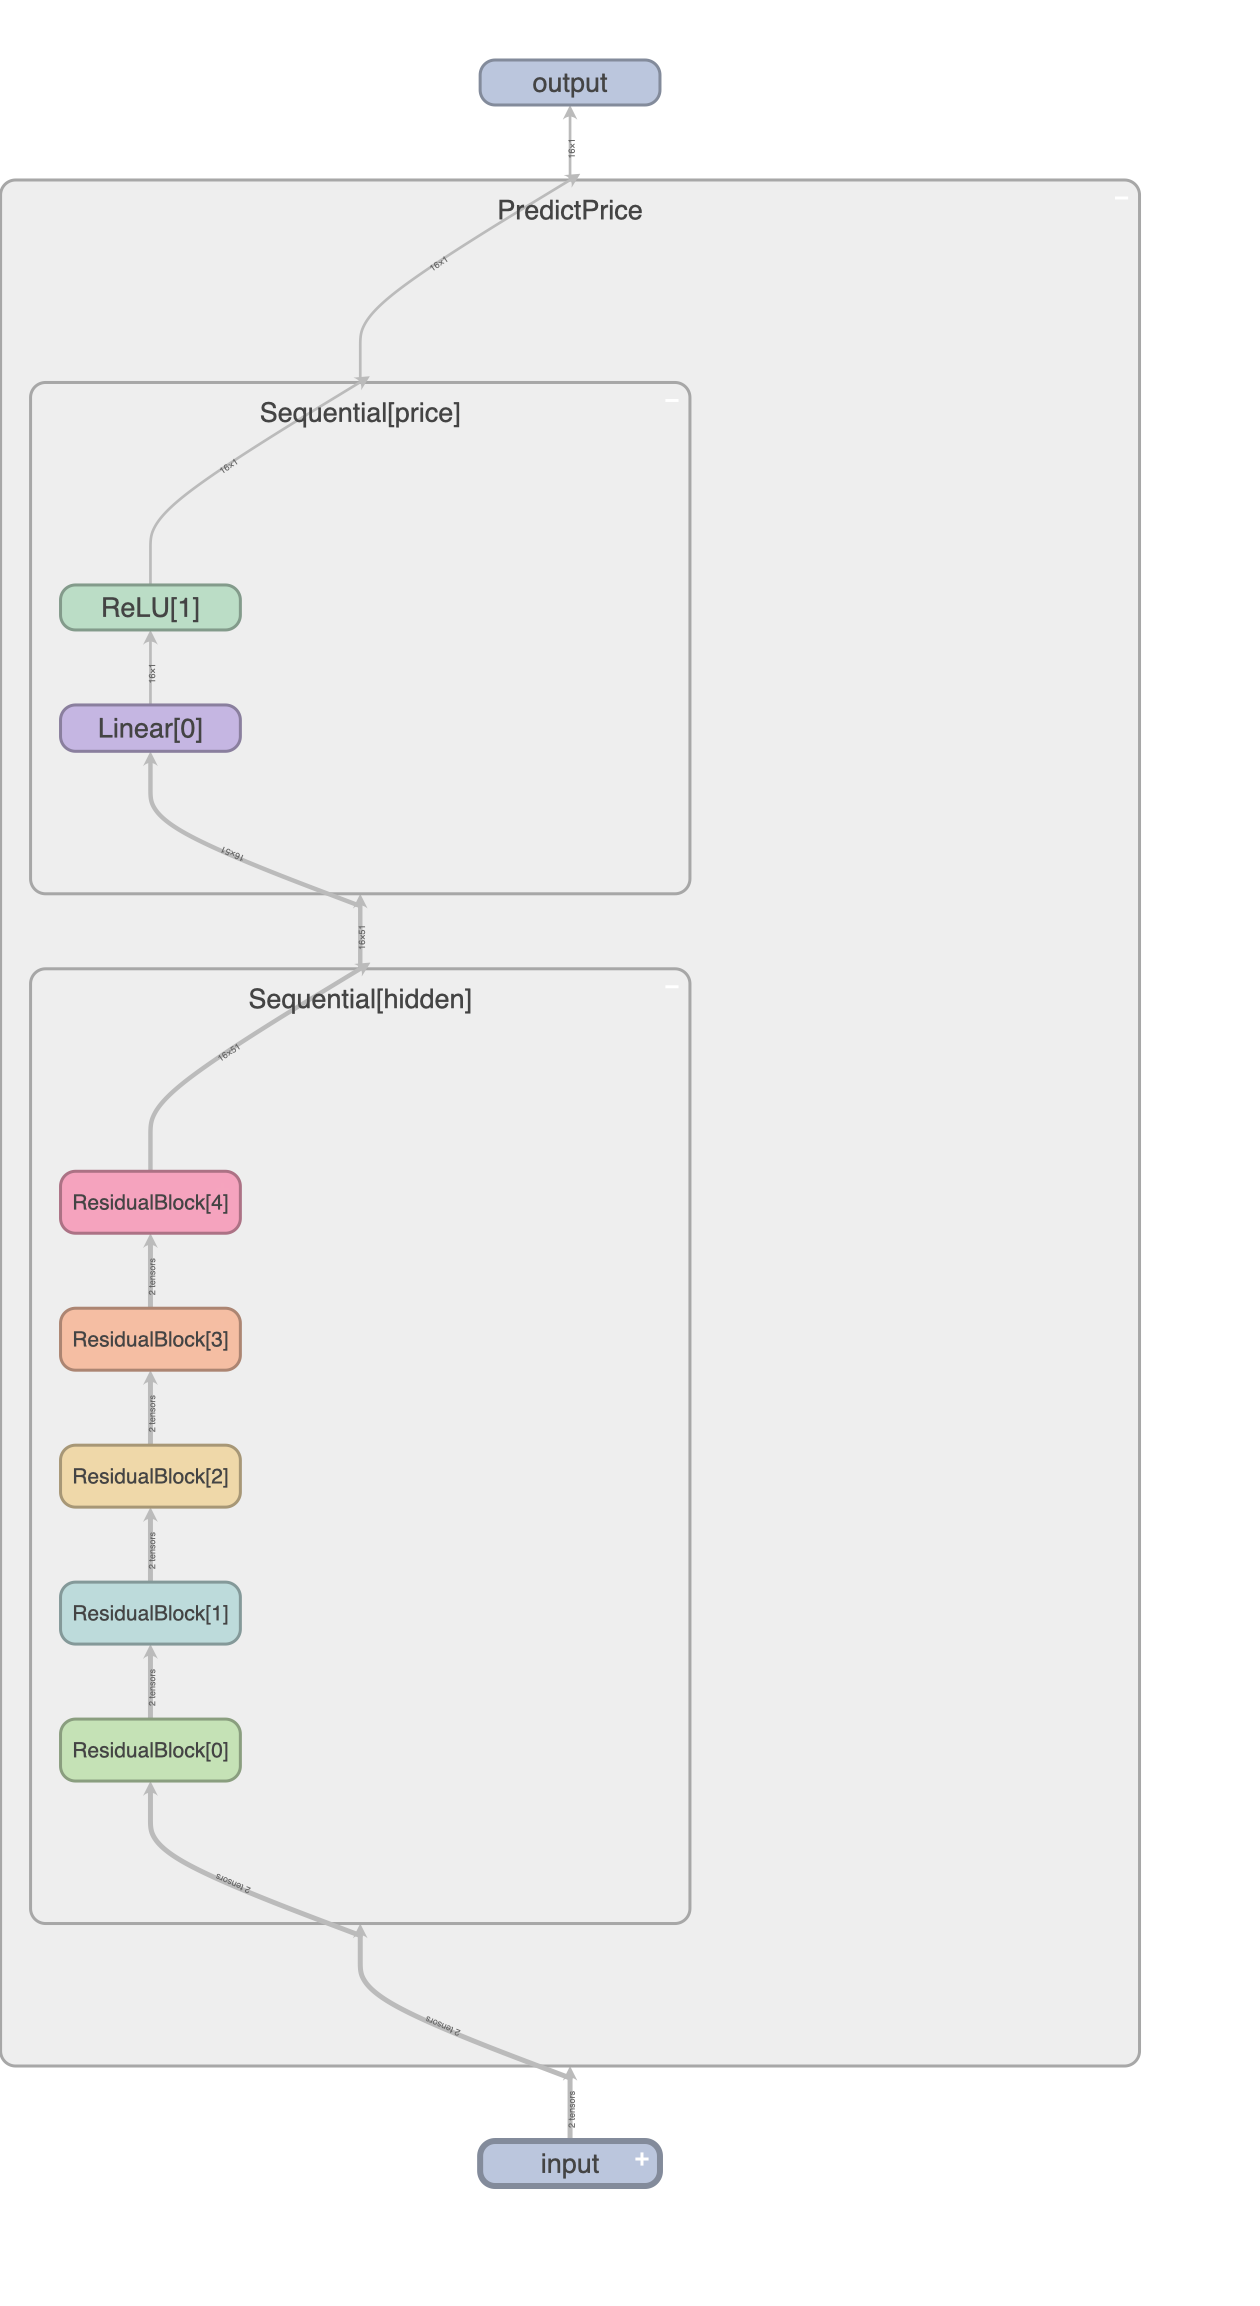
\includegraphics[width=7.5cm]{resnet_model_price}}
	\caption{Layout of residual block and network}
	\label{resnet}
\end{figure*}

\subsection{Linear Regression: Predict Status of Transactions}
Before constructing models, the correlation between the status and other attributes is obtained and depicted in figure \ref{correlation_status}. As shown in the bottom right of the graph, the correlation between actual and predicted prices are approximately -0.3. However, they were still considered model inputs because close proximity between prices increases the likelihood of a completed transaction. For example, if the predicted price is 1000 pounds/month but the actual price is 100 pounds/month, this would be considered fraud resulting in an incomplete transaction. 

\begin{figure}[!htbp]
	\centering
	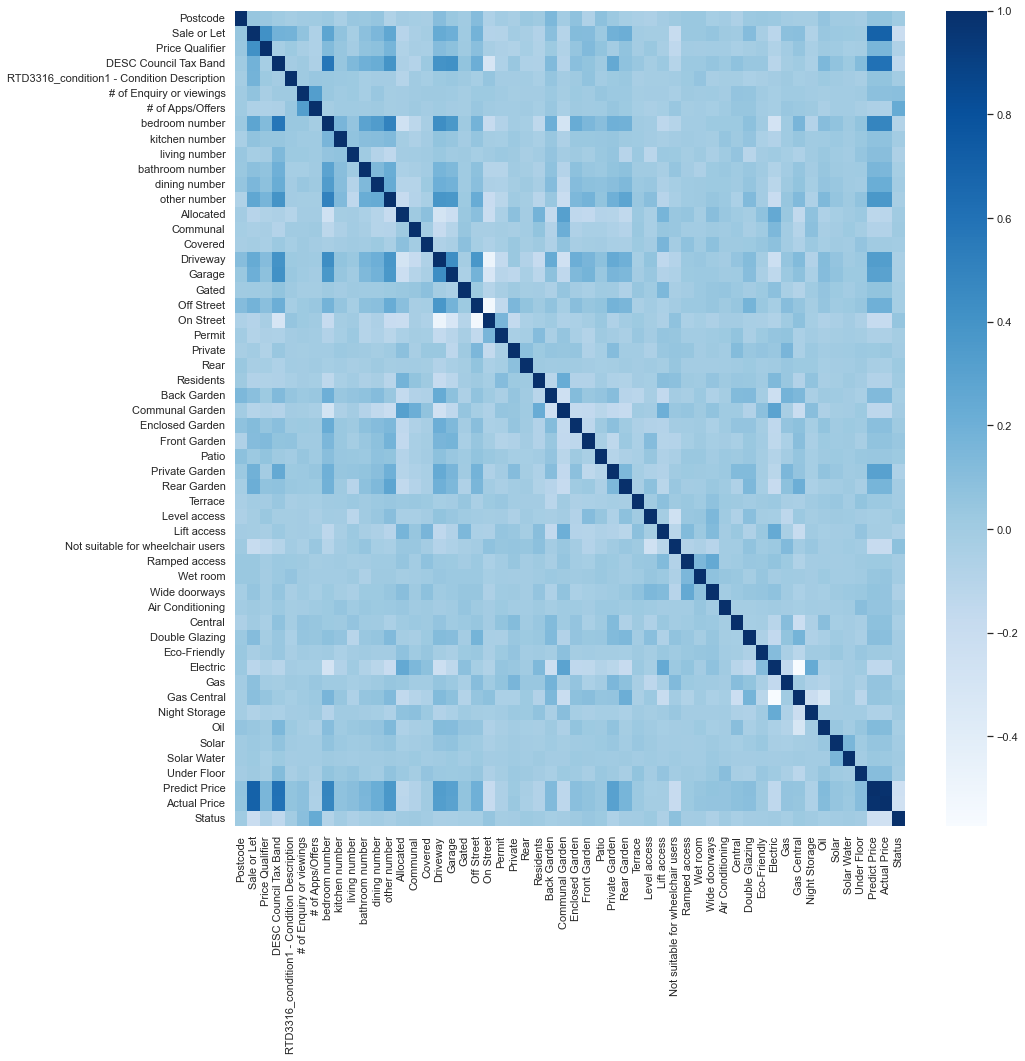
\includegraphics[width=15cm]{correlation_status}
	\caption{The correlation between the status and other attributes}
	\label{correlation_status}
\end{figure}

For the same reason as predicting prices, another linear regression model is developed to determine whether a single linear layer is sufficient for the prediction. In this case, the model is trained using two datasets, with the actual and predicted prices included in the first but excluded in the second. 

\subsection{Transfer-baesd Model: Predict Status}
There are multiple models developed previously, and their performance can be acceptable. Hence, transfer learning may be one of the practical approaches to building a model for predicting status. The selected model is the one to which WRS and outlier removal have been applied. It is loaded initially, and its parameters are frozen. Its output, along with all the attributes and actual prices, is utilized by subsequent layers for forecasting status. The complete architecture of this model is illustrated in figure \ref{transfer_layout}, and the layout of the selected model (indicated in the red rectangle) is displayed in figure \ref{basic_model_price}.

\begin{figure}[!htbp]
	\centering
	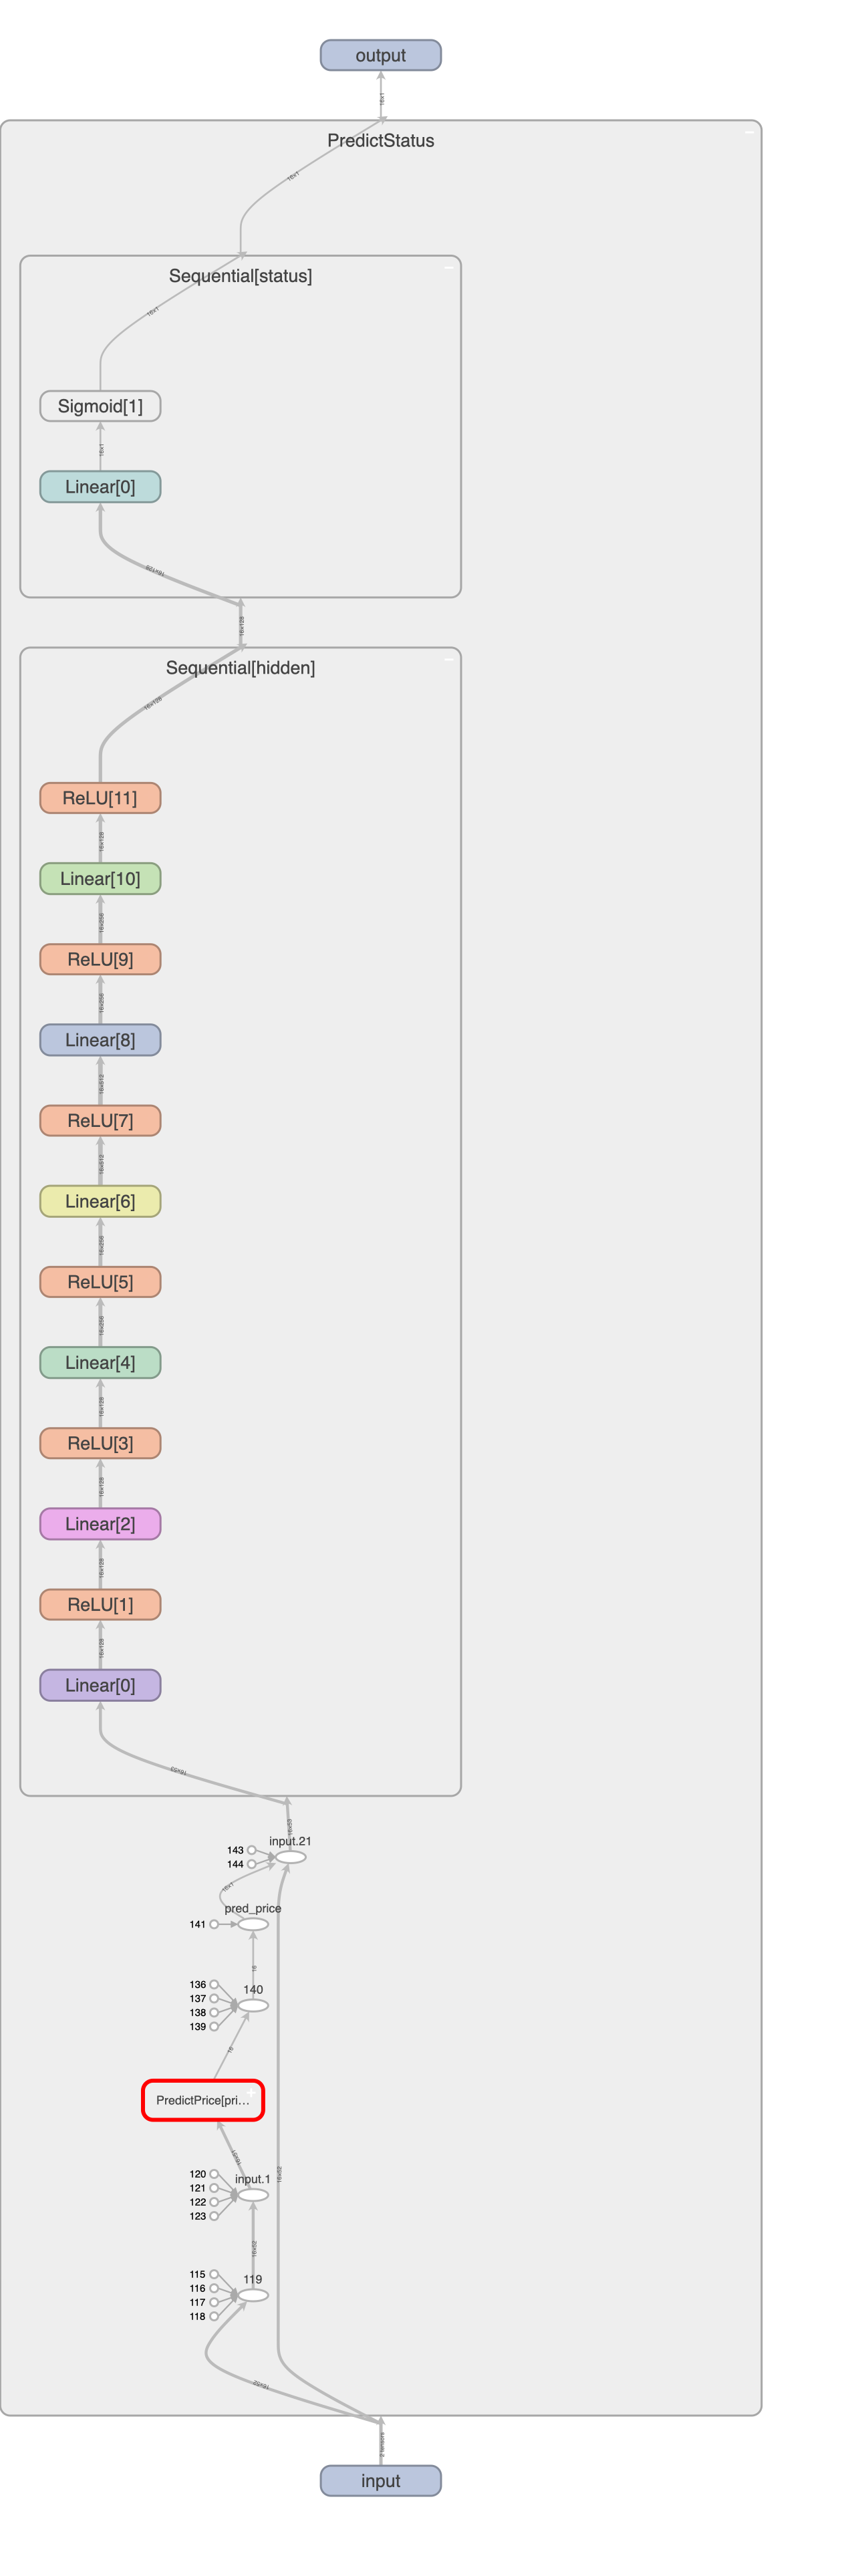
\includegraphics[height=17cm]{transfer_layout}
	\caption{The architecture of the transfer-based model for predicting status}
	\label{transfer_layout}
\end{figure}

\subsection{Basic Model: Price Included}
\label{basic_status_include}
Due to inaccurate predictions of the transfer-based model, another method to forecast status is attempted. Initially, all the features are input into the model for predicting prices, and then the predicted and actual prices are appended to the original features, resulting in a new dataset. Next, the new data is normalized, shuffled, and split into training and testing datasets. This step ensures that the inputs in this section have the same scale. Figure \ref{basic_status_layout} illustrates the structure of a new model consisting of only linear layers and activation functions, which is trained with the new dataset.

\begin{figure}[!htbp]
	\centering
	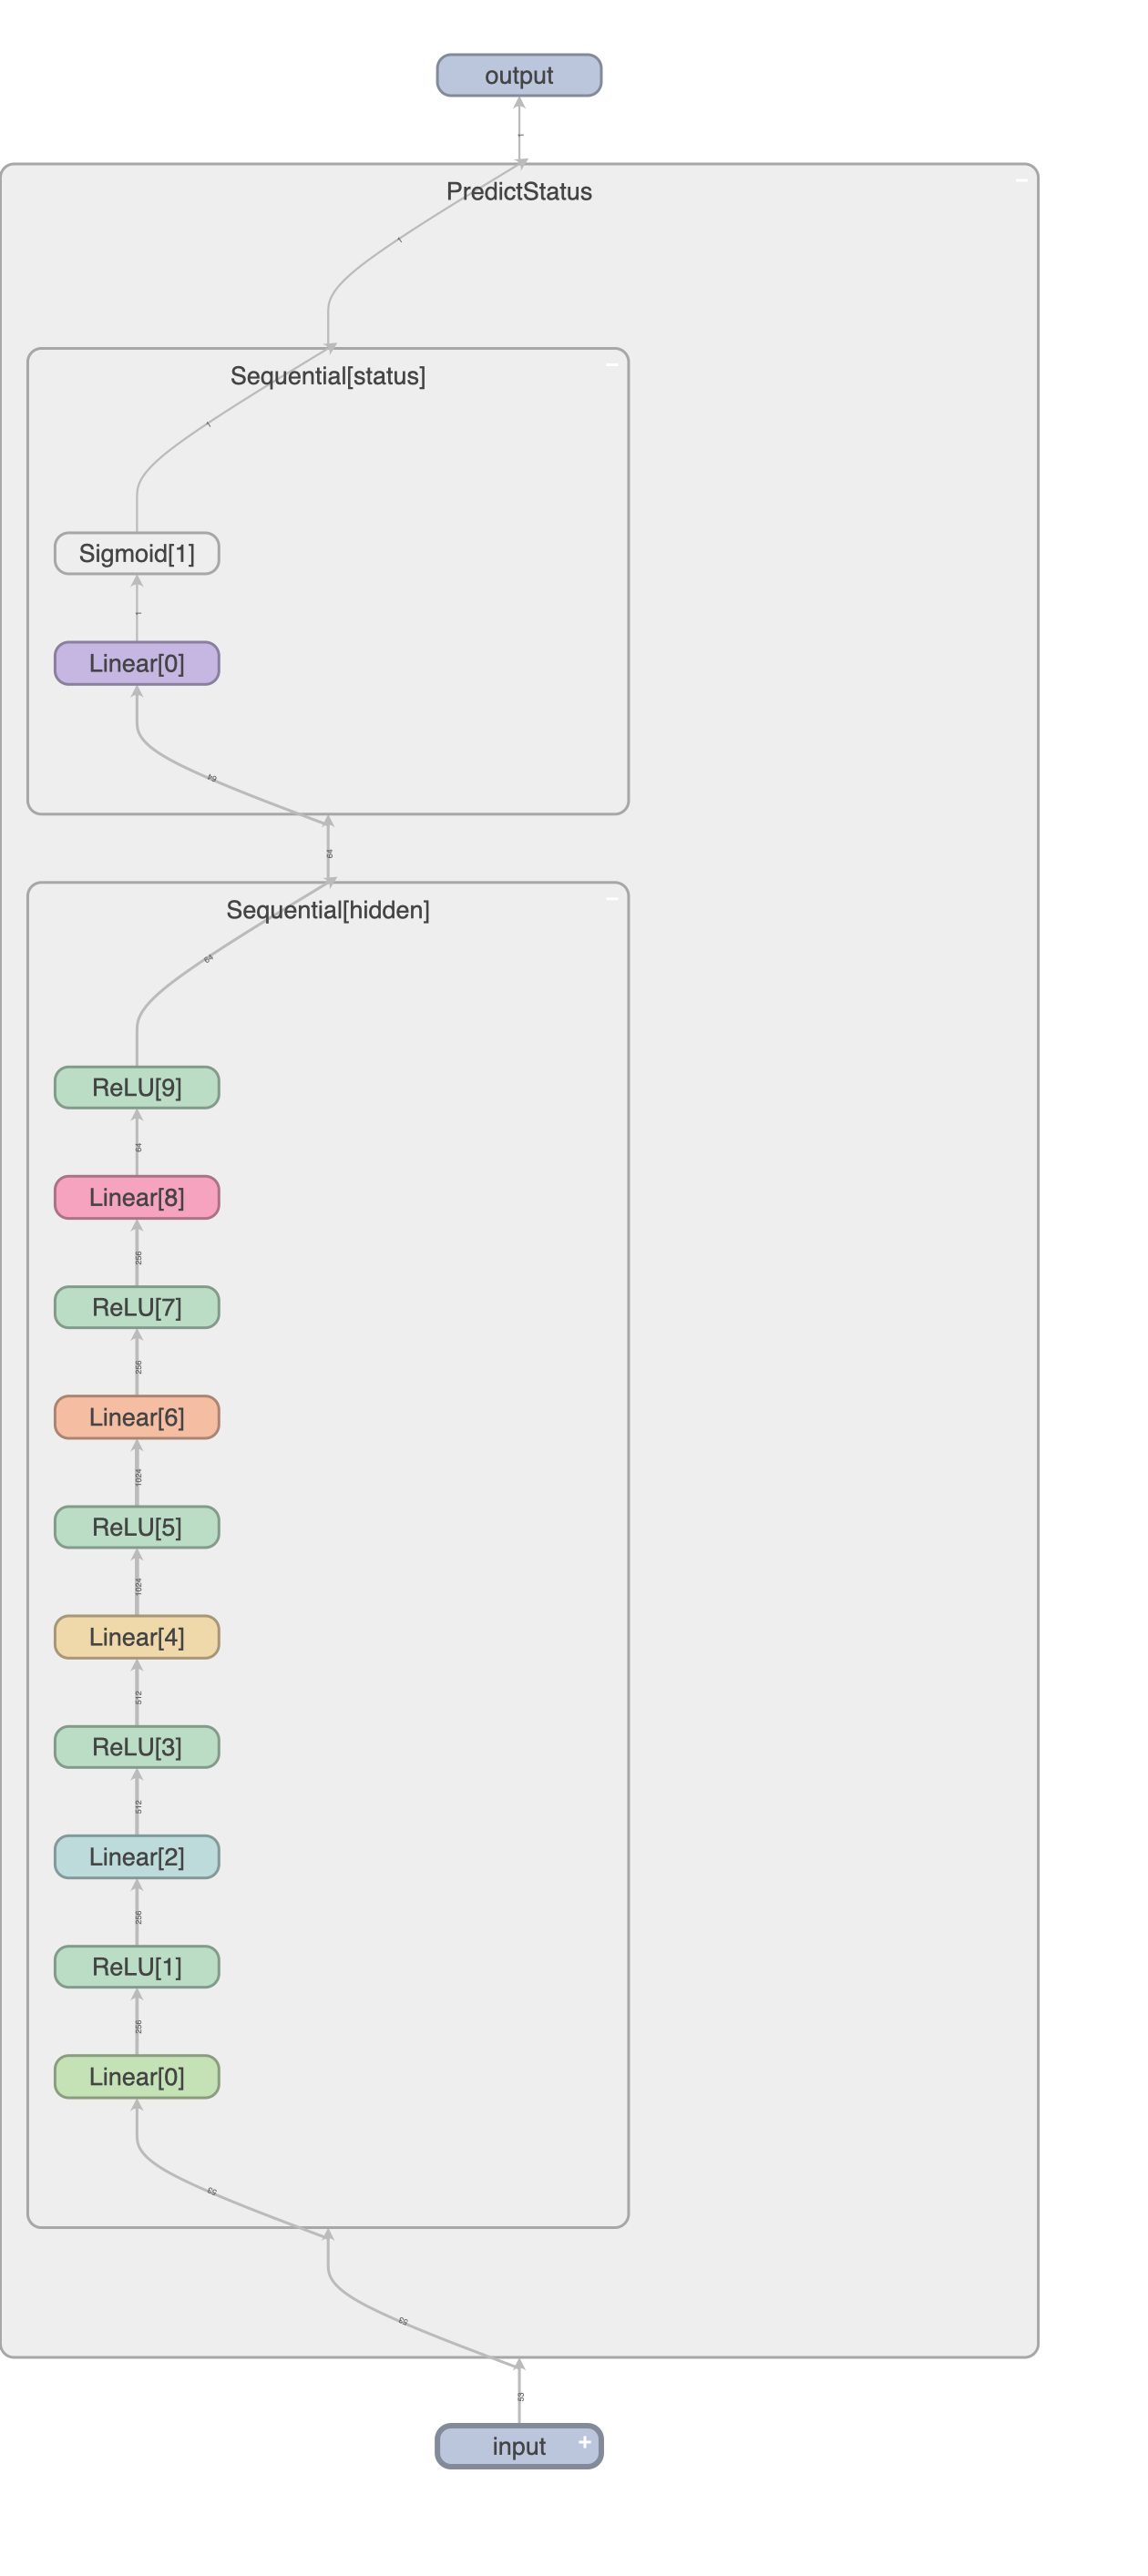
\includegraphics[height=13cm]{basic_status_layout}
	\caption{The architecture of the basic model for predicting status}
	\label{basic_status_layout}
\end{figure}

%%%%%%%%%%%%%%%%%%%%%%%%%%%%%%%%%%%%%%%%%%%%%%%%%%%%%%%%%%%%%%%%%%%
\chapter{Testing \& Experimental Results}
Comprehensive testing and analyzing were conducted throughout the development but it is documented in this separate chapter for the sake of illuatration. 

\section{Data Preprocessing}

\subsection{Handle Room Descriptions (HTML)}
There are two tests for this objective, the first test examing if the room name and its dimension can be acquiare from HTML texts and the second test focuses on if the room areas can be obtained and integrated correctly. 

\subsubsection{Acquire room name and dimension}
This test utilized two HTML texts, which are illustrated in figure \ref{html_room_info_test}. After invoking the function \textit{EweMove\_Description\_S3\_Rooms} with two snippets and retrieving the results (shown in tables \ref{html_room_info_expect_1} \& \ref{html_room_info_expect_2}), it is evident that the room names in two HTML snippets could be obtained, and the dimensions are acquired if available otherwise, the value is set to one. Therefore, this function can pass the test.

\begin{figure*}[!htbp]
	\centering
	\subfigure[Snippte 1]{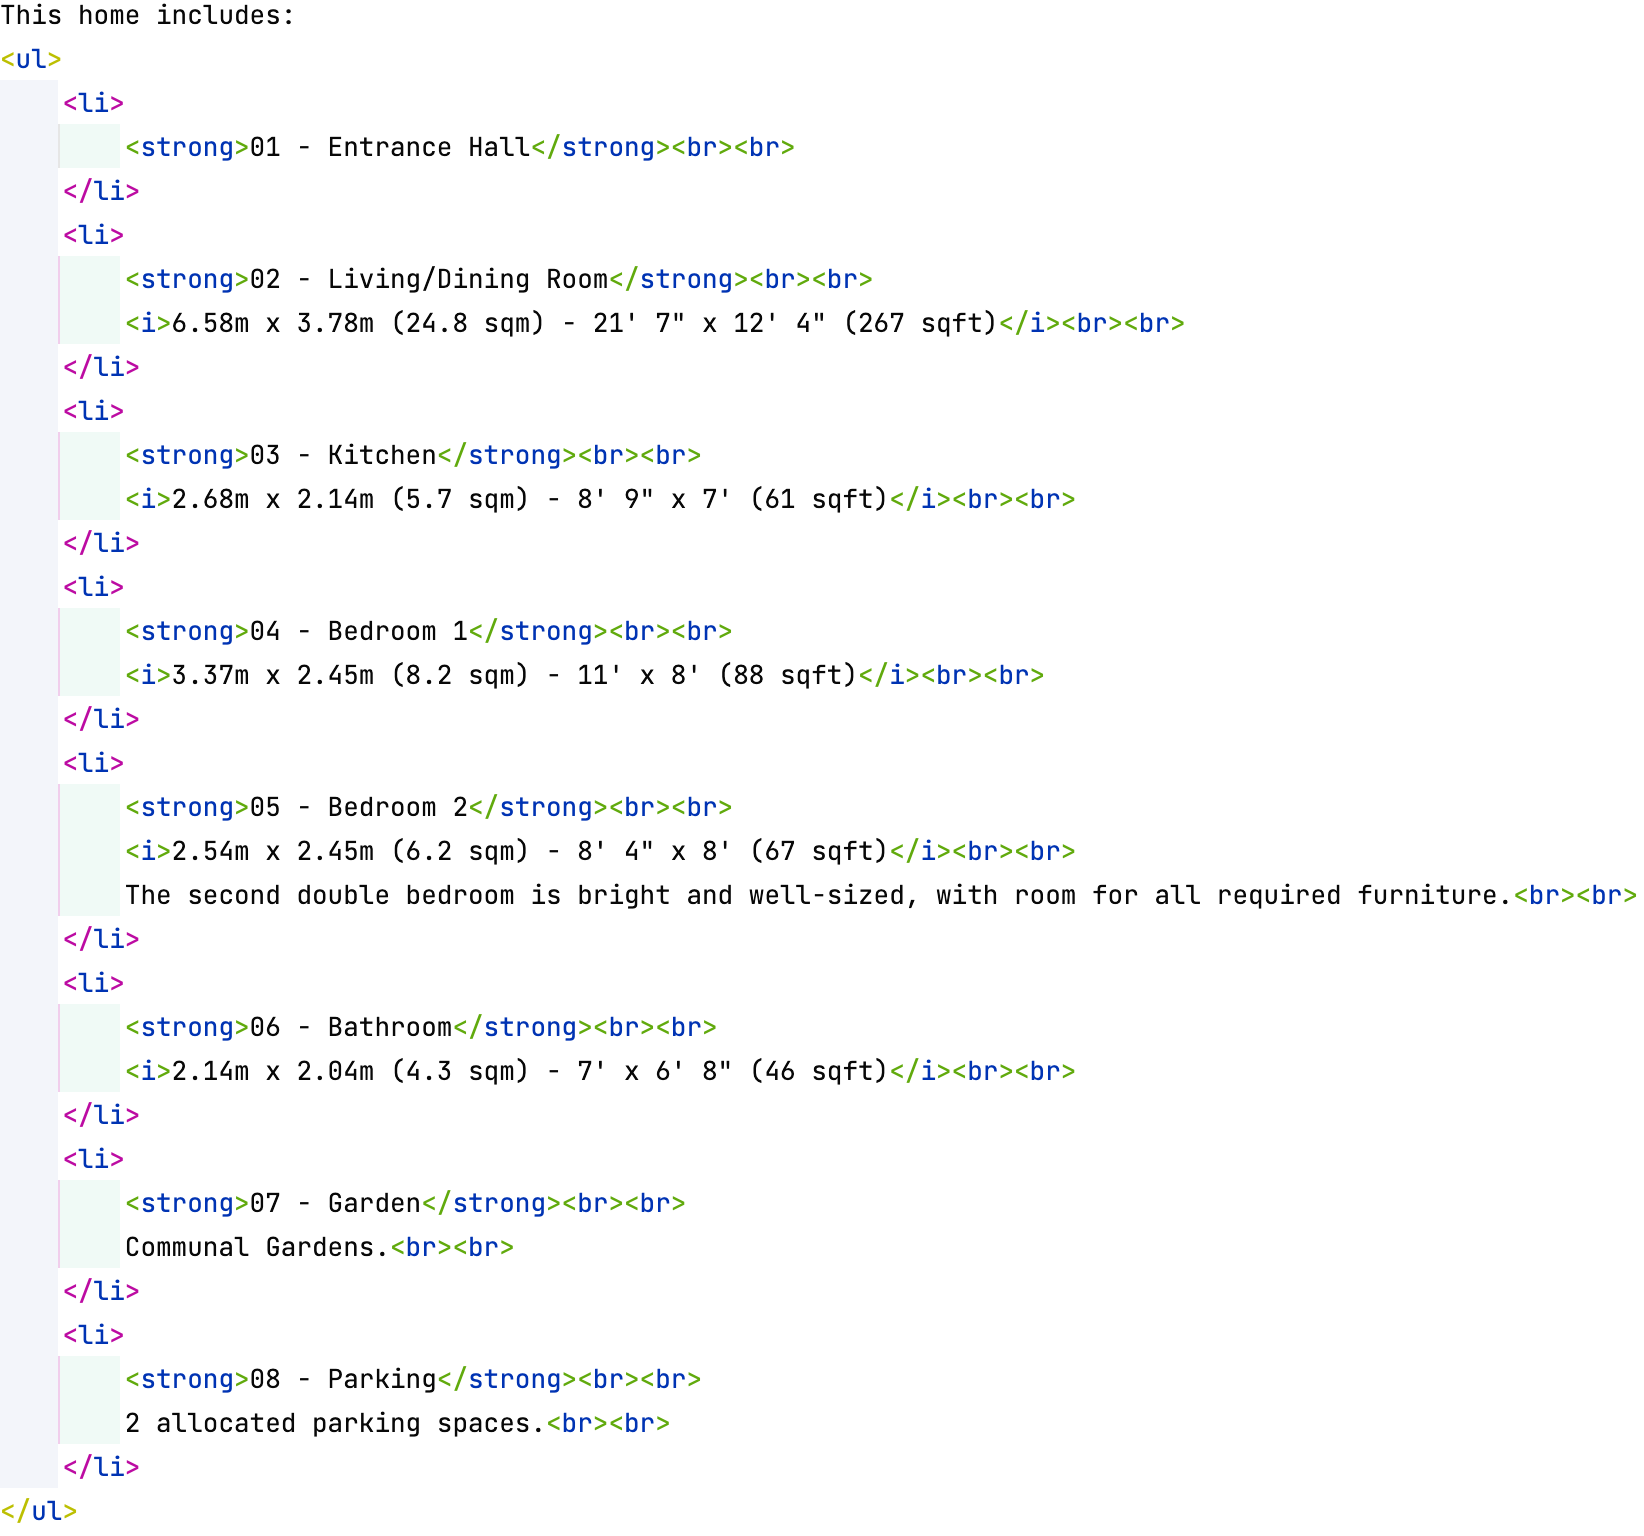
\includegraphics[width=7.5cm, height=8cm]{html_room_info_1}\label{html_room_info_test_1}}
	\hfill
	\subfigure[Snippet 2]{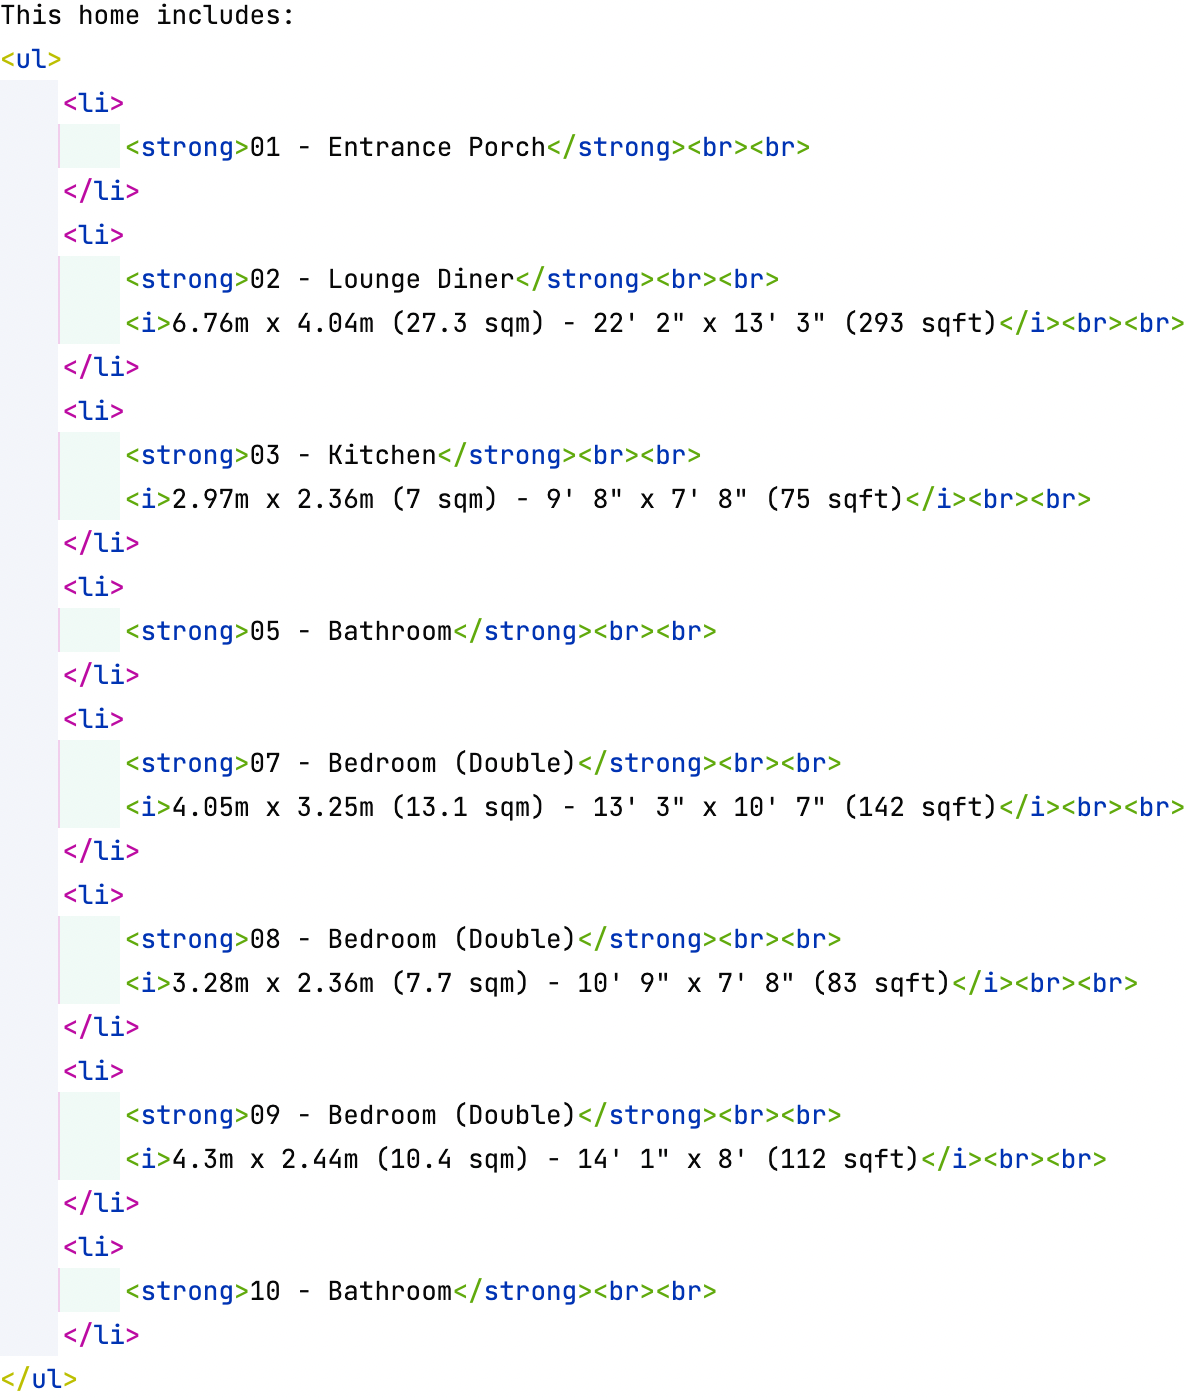
\includegraphics[width=7.5cm, height=8cm]{html_room_info_2}\label{html_room_info_test_2}}
	\caption{The HTML snippets for testing}
	\label{html_room_info_test}
\end{figure*}

\begin{table}[!htbp]
	\centering
	\caption{Information from HTML snippet in figure \ref{html_room_info_test_1}}
	\begin{tabular} {| l | l |}
		\hline
		Entrance Hall & 1\\
		\hline
		Living/Dining Room & 6.58m x 3.78m (24.8 sqm) - 21' 7" x 12' 4" (267 sqft)\\
		\hline
		Kitchen & 2.68m x 2.14m (5.7 sqm) - 8' 9" x 7' (61 sqft)\\
		\hline
		Bedroom 1 & 3.37m x 2.45m (8.2 sqm) - 11' x 8' (88 sqft)\\
		\hline
		Bedroom 2 & 2.54m x 2.45m (6.2 sqm) - 8' 4" x 8' (67 sqft)\\
		\hline 
		Bathroom & 2.14m x 2.04m (4.3 sqm) - 7' x 6' 8" (46 sqft)\\
		\hline
		Garden & 1\\
		\hline
		Parking & 1\\
		\hline
	\end{tabular}
	\label{html_room_info_expect_1}
\end{table}

\begin{table}[!htbp]
	\centering
	\caption{Information from HTML snippet in figure \ref*{html_room_info_test_2}}
	\begin{tabular} {| l | l |}
		\hline
		Entrance Porch & 1\\
		\hline
		Lounge Diner & 6.76m x 4.04m (27.3 sqm) - 22' 2" x 13' 3" (293 sqft)\\
		\hline
		Kitchen & 2.97m x 2.36m (7 sqm) - 9' 8" x 7' 8" (75 sqft)\\
		\hline
		Bathroom & 1\\
		\hline
		Bedroom (Double) & 4.05m x 3.25m (13.1 sqm) - 13' 3" x 10' 7" (142 sqft)\\
		\hline 
		Badroom (Double) & 3.28m x 2.36m (7.7 sqm) - 10' 9" x 7' 8" (83 sqft)\\
		\hline
		Bedroom (Double) & 4.3m x 2.44m (10.4 sqm) - 14' 1" x 8' (112 sqft)\\
		\hline
		Bathroom & 1\\
		\hline
	\end{tabular}
	\label{html_room_info_expect_2}
\end{table}

\subsubsection{Generalize room information}
The data obtained from HTML texts (figure \ref{html_room_info_test}) is used to access the behavior of \textit{ExtractRooms}, particularly its member function \textit{get\_rooms}. During testing, the selected type is the bedroom, and all the operations of \textit{get\_room} are inspected. Additionally, the other rooms are used to test function \textit{get\_rest\_rooms}. 
\\

The results of calling \textit{get\_rooms} are displayed in tables \ref{bedroom_info_split} and \ref{bedroom_info_all}. It is obvious that all the bedrooms and their respective areas in tables \ref{html_room_info_expect_1} and \ref{html_room_info_expect_2} are successfully extracted. Moreover, the numerical values could also be obtained without error if the operations are appropriately configured. These behaviors demonstrates that the functionality and design are identical. In addition, the result of invoking \textit{get\_rest\_rooms} is displayed in table \ref{other_room_info}. It is clear that there is no statistical inconsistency using the information from tables \ref{html_room_info_expect_1} and \ref{html_room_info_expect_2}, hence this function can pass the test. 

\begin{table}[!htbp]
	\centering
	\captionof{table}{Room information (\textit{split})}
	\label{bedroom_info_split}
	\begin{tabular}{| c | c | c | c |}
		\hline
		& Bedroom 1 & Bedroom 2 & Bedroom 3 \\
		\hline
		0 & 8.2 & 6.2 & 0.0 \\
		\hline
		1 & 13.1 & 7.7 & 10.4 \\
		\hline
	\end{tabular}
\end{table}

\begin{table*}[!htbp]
	\centering
	\caption{Bedroom information integrated by different operations}
	\label{bedroom_info_all}
	\subtable[Mean]{
		\begin{tabular}{| c | c |}
			\hline
			& Average area \\ 
			\hline
			0 & 7.2 \\
			\hline
			1 & 10.4 \\ 
			\hline
		\end{tabular}
		\label{bedroom_info_mean}
	}
	\hfill
	\subtable[Sum]{
		\begin{tabular}{| c | c |}
			\hline
			& Total area \\ 
			\hline
			0 & 14.4 \\
			\hline
			1 & 31.2 \\ 
			\hline
		\end{tabular}
		\label{bedroom_info_sum}
	}
	\hfill
	\subtable[Number]{
		\begin{tabular}{| c | c |}
			\hline
			& Number of rooms \\ 
			\hline
			0 & 2 \\
			\hline
			1 & 3 \\ 
			\hline
		\end{tabular}
		\label{bedroom_info_number}
	}
	\subtable[Other rooms]{
		\begin{tabular}{| c | c | c |}
			\hline
			& Number & Area \\
			\hline
			0 & 6 & 34.8 \\
			\hline
			1 & 5 & 34.3 \\
			\hline
		\end{tabular}
		\label{other_room_info}
	}
\end{table*}

\subsection{Manipulate Categorical Keywords}
The data utilized for this test is displayed in figure \ref{parking_dataset}. Initially, an invalid feature, \textit{Distance to School}, is input into the function \textit{get\_feature\_types}, and the feature is then set to \textit{parking}. With the same data, the member function \textit{get\_feature\_num} is evaluated.
\\

In the initial test, an exception can be thrown if an invalid feature is entered, in this case, \textit{Distance to School}. Next, the result of calling function \textit{get\_feature\_types} is shown in table \ref{parking_types}. Since there are ten properties in the snippets and six keywords in total, this table has ten rows and six columns which is correct, and its elements are consistent with the dataset snippet. For the first property with an \textbf{allocated} \textbf{off-street} parking space for \textbf{residents}, the three keywords in the first row are set to one while the others are zero, and this conclusion holds true for the remaining properties. In addition, the number of keywords associated with each property can be obtained accurately by calling \textit{get\_feature\_num}. 

\begin{table}[!htbp]
	\centering
	\caption{The keywords for each property}
	\label{parking_types}
	\begin{tabular}{| c | c | c | c | c | c | c |}
		\hline
		& Allocated & Driveway & Garage & Off Street & On Street & Residents\\
		\hline
		0 & 1 & 0 & 0 & 1 & 0 & 1 \\ 
		\hline
		1 & 0 & 0 & 0 & 0 & 0 & 0 \\
		\hline
		2 & 0 & 0 & 0 & 0 & 1 & 0 \\
		\hline
		3 & 0 & 0 & 0 & 0 & 0 & 0 \\
		\hline
		4 & 0 & 1 & 1 & 1 & 0 & 0 \\
		\hline
		5 & 0 & 0 & 0 & 0 & 0 & 0 \\
		\hline
		6 & 0 & 1 & 1 & 1 & 0 & 0 \\
		\hline
		7 & 0 & 1 & 0 & 0 & 0 & 0 \\
		\hline
		8 & 0 & 1 & 1 & 0 & 0 & 0 \\
		\hline
		9 & 0 & 1 & 1 & 0 & 0 & 0 \\
		\hline
	\end{tabular}
\end{table}

\subsection{Manage Outliers}
During preprocessing, both filling the mean value and removing outliers are attempted. The distributions of the prices after applying two methods are demonstrated in figures \ref{price_filled} and \ref{price_removed}. For filling the average value, it is apparent that the left-hand spike is diminished, meaning that there is no price of zero. A new peak in the middle suggests that the original distribution has been modified. If zero prices are removed, the peak on the left would also be reduced, and the distribution would remain unchanged. 
\\

\begin{figure}[!htbp]
	\centering
	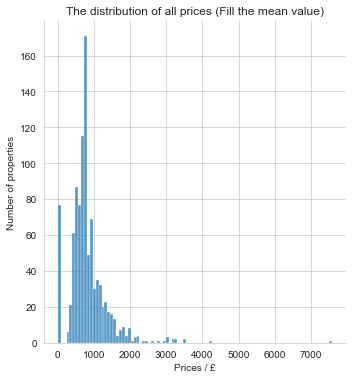
\includegraphics[height=4cm]{price_all_mean}
	\caption{The distribution of prices with mean value filled}
	\label{price_filled}
\end{figure}

Therefore, removing zero prices is applied to create input datasets for models as it retains the original distribution, whereas filling the mean value causes the data alternation. Consequently, the model will learn more from average, which results in poor performance. 

\begin{figure*}[h]
	\centering
	\subfigure[Sale Prices]{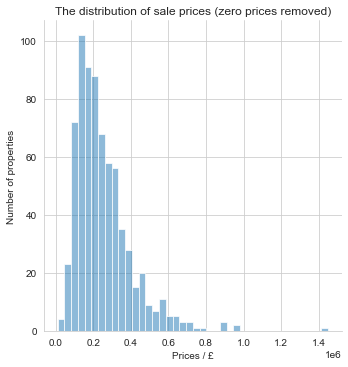
\includegraphics[height=4cm]{price_sale_remove}\label{price_sale_remove}}
	\hfil
	\subfigure[Rental Prices]{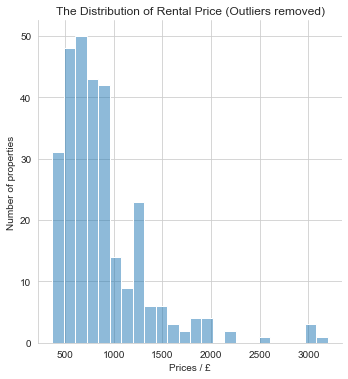
\includegraphics[height=4cm]{price_rental_remove}\label{price_rental_remove}}
	\caption{The distribution of prices with zero prices removed}
	\label{price_removed}
\end{figure*}

\subsection{Create Input Dataset}
The first step in evaluating the behavior of this class is to determine if the categorical features are encoded, and the second test is to inspect whether the missing values are eliminated.
\\

For general information, the first ten rows after preprocessing and their corresponding rows in the original dataset are displayed in figure \ref{general_info}. The categorical features, such as postcode and council tax band, are encoded as numerical values allowing the first test to be passed. In addition, it is evident that the indices in the new dataset are not continuous, indicating that the rows with missing values have been removed. Hence it can pass the second test. 

\begin{figure*}[!htbp]
	\centering
	\subfigure[Original dataset]{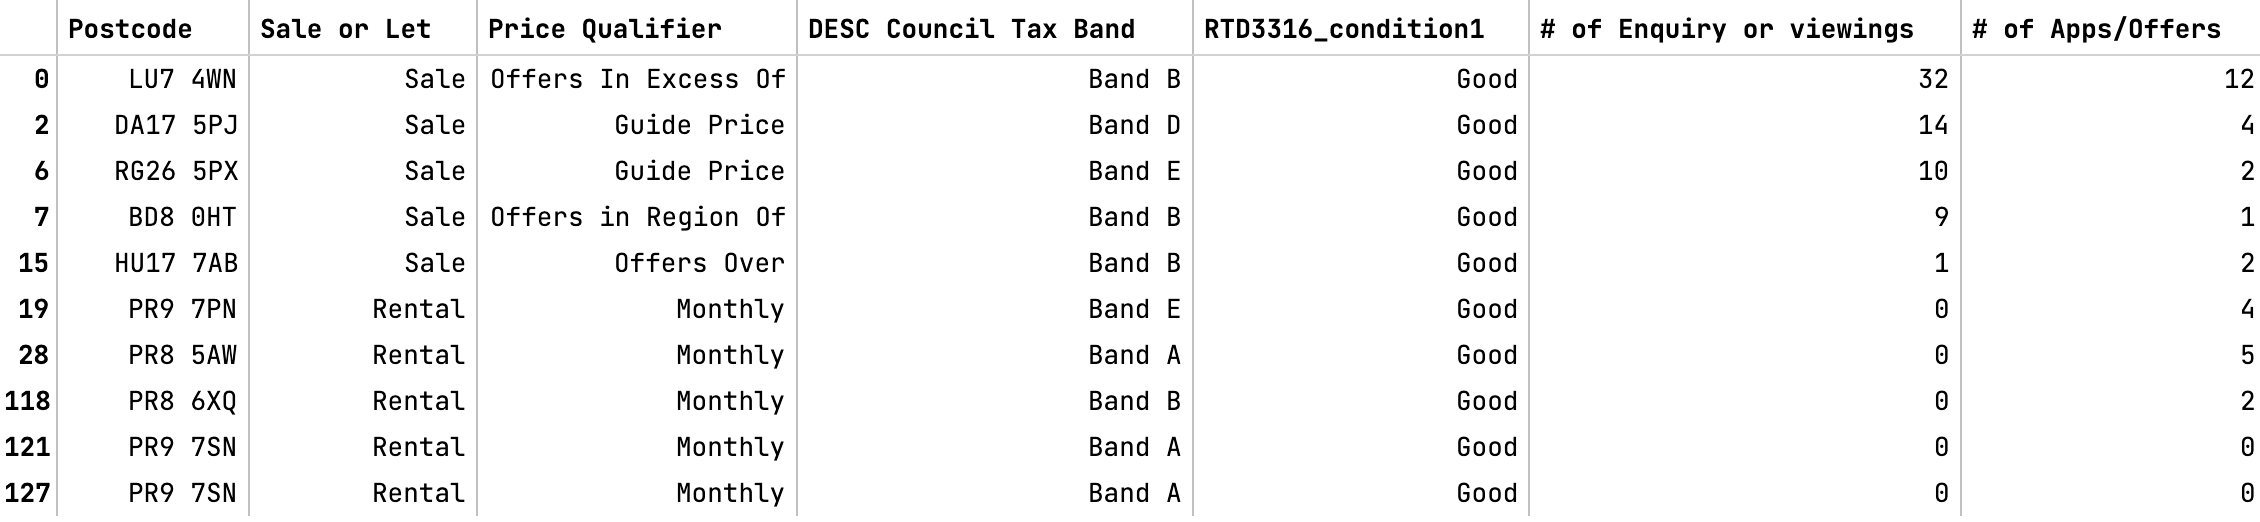
\includegraphics[width=\linewidth]{general_raw}\label{general_raw}}
	\subfigure[Preprocessed dataset]{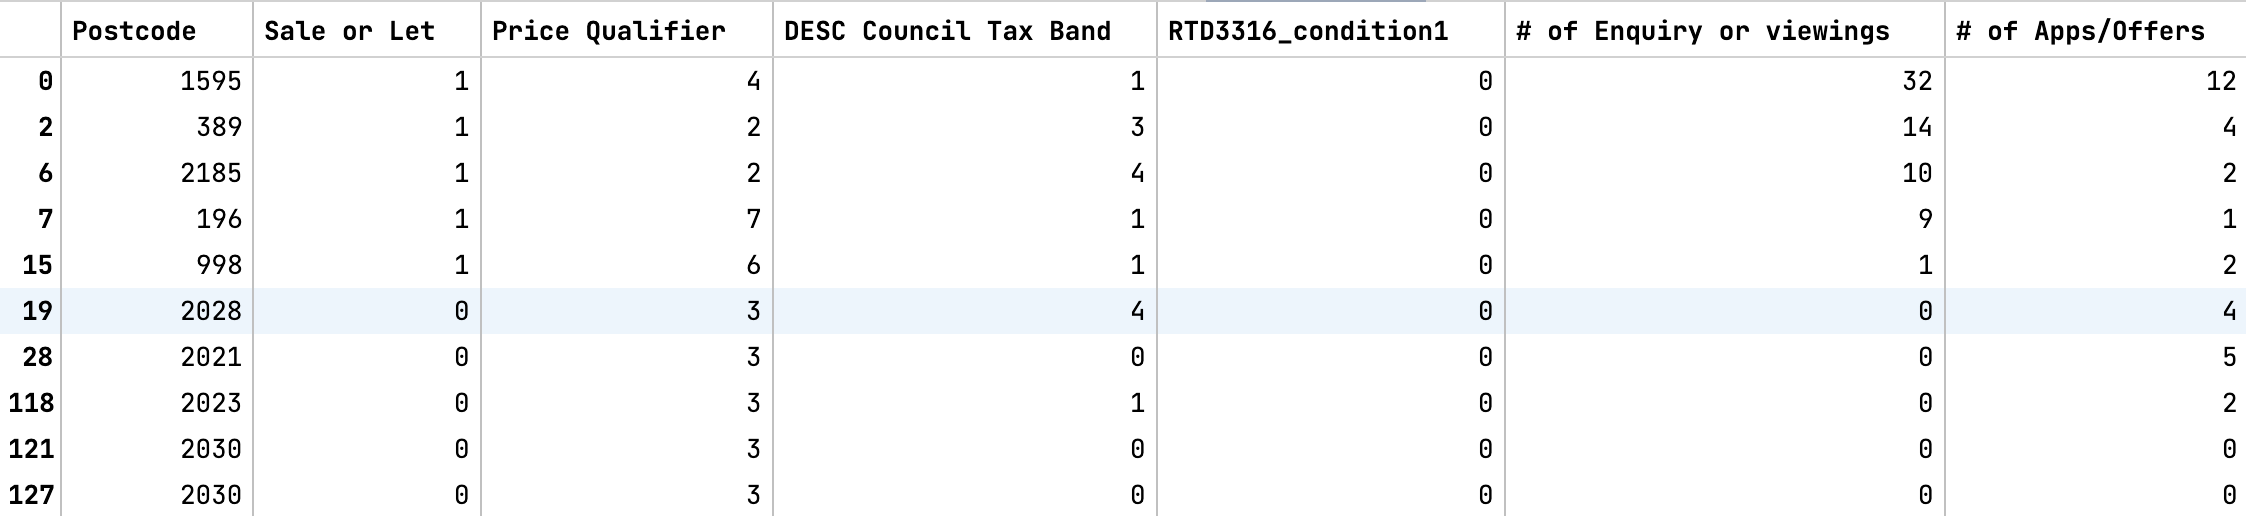
\includegraphics[width=\linewidth]{general_input}\label{general_input}}
	\caption{Comparsion between original and preprocessed dataset}
	\label{general_info}
\end{figure*}

\section{Model Construction}

\subsection{Basic Model: Output Sale Status and Price}
The training and validation losses against epochs for each fold are displayed in figure \ref{sale_fold_5}. For fold zero, the model is overfitting as the training loss is approximately the same after 60 epochs, whereas the validation loss is increasing. If the training stops earlier, then the performance of this model may be the best. For fold one, the model is underfitting as the validation loss keeps decreasing and its performance might be better if it is trained for more epochs. For the next two folds, the performance of the models are the best and should be selected for testing. The model trained from the last fold does not learn anything since both training and validation loss oscillate significantly. 
\\

\begin{figure*}[!htbp]
	\centering
	\subfigure[Fold 0]{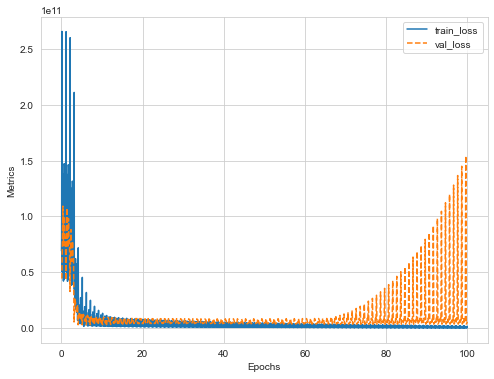
\includegraphics[width=5cm]{sale_fold_5_0}\label{sale_fold_5_0}}
	\hfill
	\subfigure[Fold 1]{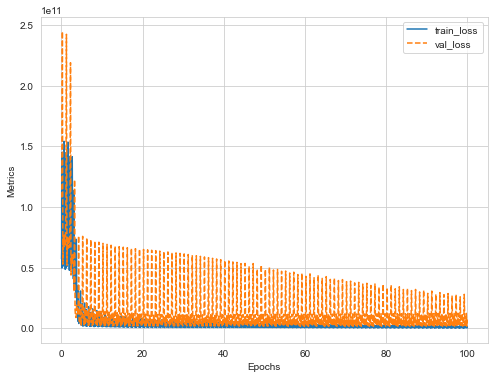
\includegraphics[width=5cm]{sale_fold_5_1}\label{sale_fold_5_1}}
	\hfill
	\subfigure[Fold 2]{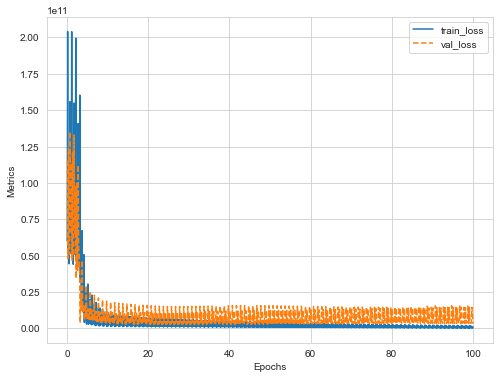
\includegraphics[width=5cm]{sale_fold_5_2}\label{sale_fold_5_2}}
	\hfil
	\subfigure[Fold 3]{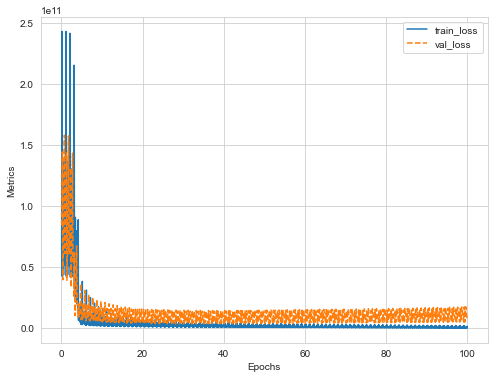
\includegraphics[width=5cm]{sale_fold_5_3}\label{sale_fold_5_3}}
	\hfil
	\subfigure[Fold 4]{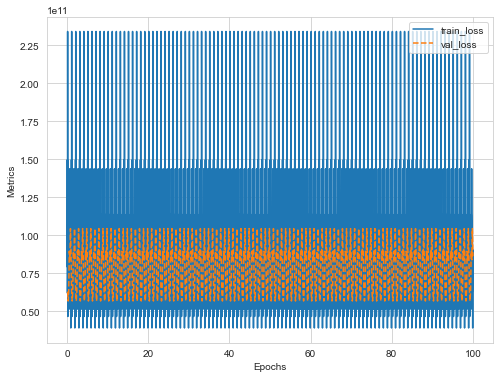
\includegraphics[width=5cm]{sale_fold_5_4}\label{sale_fold_5_4}}
	\caption{The training \& validation loss for different folds}
	\label{sale_fold_5}
\end{figure*}

Based on the performance plot, the model trained in fold three is selected. The first ten predictions and true values are shown in table \ref{first_model_predictions}. It is evident that the model only predict one for status regardless of the truth values, whereas the predicted prices are better.  
\\

The metrics for price prediction are as follows, $MSE = 7559964776$ and $R^2 = 0.54$. Comparing this model to the linear regression model demonstrates that the neural network is able to extract patterns from the dataset, resulting in superior performance. 
\\

Figure \ref{confusion_matrix_basic_model} illustrates the confusion matrix of predicting completeness, from which the accuracy, precision, recall, and F1 score are calculated to be 0.638, 0.638, 1, and 0.78, respectively. 
\\

\begin{figure}[!htbp]
	\centering
	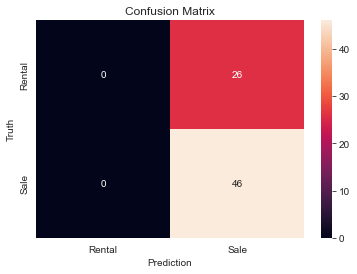
\includegraphics[width=9cm]{confusion_matrix_basic_model}
	\caption{The confusion matrix of the basic model}
	\label{confusion_matrix_basic_model}
\end{figure}

One of the possible causes of the error results are loss functions. The completeness is either zero or one, hence the BCE loss is utilized. For the prices which is greater than zero, the MSE loss is applied. As the model outputs both completeness and prices, the BCE and MSE loss are added to produce a total loss that is then used for backpropagation. However, the BCE loss is negligible compared with MSE loss. Therefore, the total loss results in the model learning more about predicting prices, while completeness is ignored. Additionally, the price is not input into the model, despite being one of the most important factors in real transactions and thus contributing to the incorrect predictions of the status.

\begin{table}[!htbp]
	\centering
	\caption{Comparison between truth and model predictions}
	\label{first_model_predictions}
	\begin{tabular}{| c | c | c | c | c |}
		\hline
		Completed & Price & Predicted Status & Predicted Price & Price error  / \%\\ 
		\hline
		1 & 675000 & 1 & 600810 & 10.99 \\
		\hline
		0 & 80000 & 1 & 36130 & 70.16 \\
		\hline
		0 & 90000 & 1 & 53198 & 40.89  \\
		\hline
		0 & 295000 & 1 & 253552 & 14.05  \\
		\hline
		0 & 105000 & 1 & 105753 & 0.72  \\ 
		\hline
		1 & 270000 & 1 & 297239 & 10.09  \\
		\hline
		0 & 115000 & 1 & 124108 & 7.92  \\
		\hline
		1 & 600000 & 1 & 528918 & 11.85  \\
		\hline
		1 & 4000000 & 1 & 376152 & 5.96  \\
		\hline
		0 & 125000 & 1 & 157276 & 25.82  \\
		\hline
	\end{tabular}
\end{table}

\subsection{Linear Regression: Predict Price}
The training and validation losses of this model are depicted in figure \ref{linear_regression_fold_5}, and the model trained in fold two has been chosen for evaluation since it has the lowest validation loss. 
\\
\begin{figure*}[!htbp]
	\centering
	\subfigure[Fold 0]{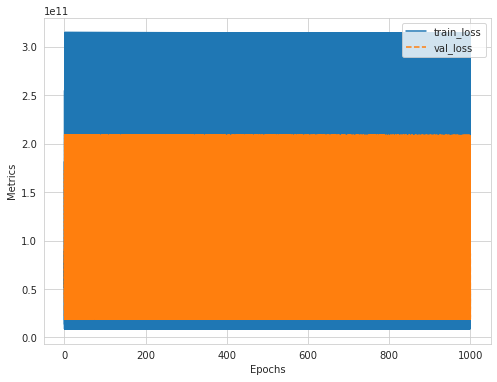
\includegraphics[width=5cm]{linear_regression_fold_0}\label{linear_regression_fold_0}}
	\hfill
	\subfigure[Fold 1]{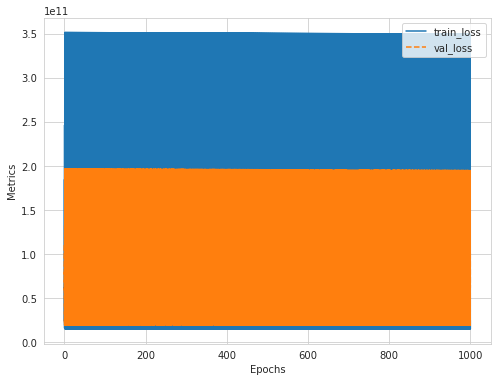
\includegraphics[width=5cm]{linear_regression_fold_1}\label{linear_regression_fold_1}}
	\hfill
	\subfigure[Fold 2]{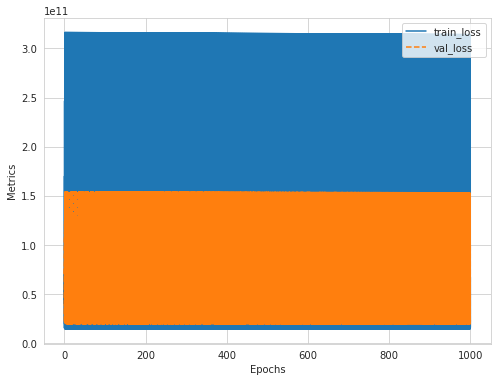
\includegraphics[width=5cm]{linear_regression_fold_2}\label{linear_regression_fold_2}}
	\hfil
	\subfigure[Fold 3]{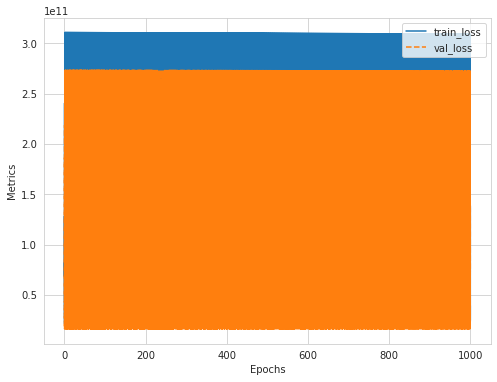
\includegraphics[width=5cm]{linear_regression_fold_3}\label{linear_regression_fold_3}}
	\hfil
	\subfigure[Fold 4]{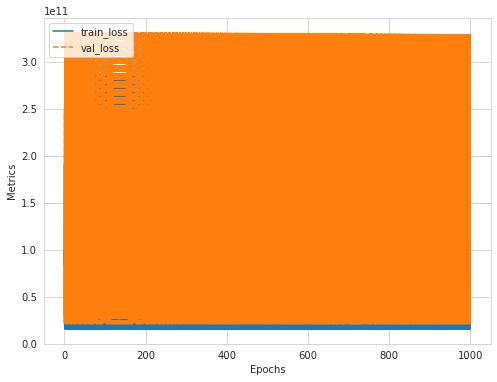
\includegraphics[width=5cm]{linear_regression_fold_4}\label{linear_regression_fold_4}}
	\caption{The training \& validation loss for different folds (linear regression model)}
	\label{linear_regression_fold_5}
\end{figure*}

\begin{table}[!htbp]
	\centering
	\caption{Comparison between truth and model predictions}
	\label{linear_regression_predictions}
	\begin{tabular}{| c | c | c |}
		\hline
		Predicted Price & Price & Price Error  / \%\\ 
		\hline
		940 & 695 & 35.37 \\
		\hline
		4150 & 350000 & 98.81 \\
		\hline
		1790 & 130000 & 98.62 \\
		\hline
		-2101 & 475 & 542.46 \\
		\hline
		1829 & 105000 & 98.25 \\
		\hline
		3058 & 450000 & 99.32 \\
		\hline
		-4289 & 460 & 1032.47 \\
		\hline
		855 & 325000 & 99.74 \\
		\hline
		3255 & 585000 & 99.44 \\
		\hline
		1071 & 900 & 19.10 \\
		\hline
	\end{tabular}
\end{table}

The first ten predictions and the actual prices are displayed in table \ref{linear_regression_predictions}, and it is evident that there are significant differences between the predictions and the truth. Moreover, the model's metrics are as follows, $MSE = 66601086343$ and $R^2 = -0.91$. These results demonstrate that a linear regression model cannot extract patterns from the dataset and that neural networks with multiple layers are compulsory.

\subsection{Basic Model: Predicting Prices}
Initially, the training \& validation losses of this model is displayed in figure \ref{all_full_epoch_1000}, and the model from fold one is selected for the evaluation because of its performance. The first ten predictions are shown in table \ref{first_model_predictions}, and the metrics of this model are as follows, $MSE = 4918700785$, and $R^2 = 0.85$. 

\begin{figure*}[!htbp]
	\centering
	\subfigure[Fold 0]{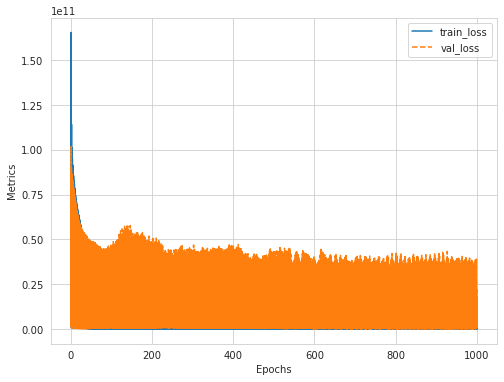
\includegraphics[width=5cm]{all_full_epoch_1000_fold_0}}
	\hfill
	\subfigure[Fold 1]{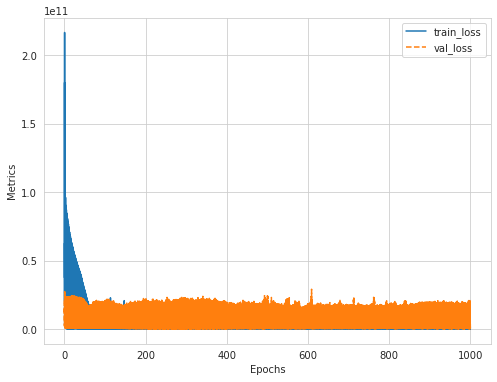
\includegraphics[width=5cm]{all_full_epoch_1000_fold_1}}
	\hfill
	\subfigure[Fold 2]{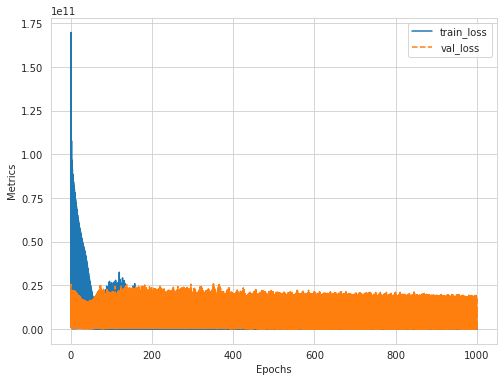
\includegraphics[width=5cm]{all_full_epoch_1000_fold_2}}
	\hfil
	\subfigure[Fold 3]{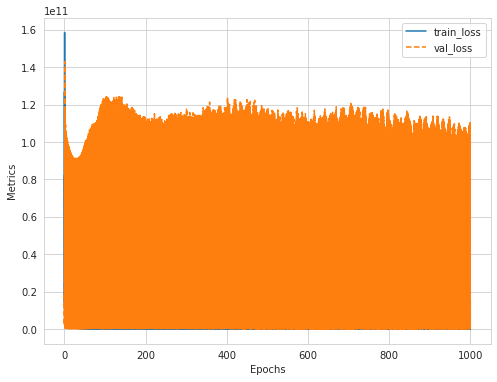
\includegraphics[width=5cm]{all_full_epoch_1000_fold_3}}
	\hfil
	\subfigure[Fold 4]{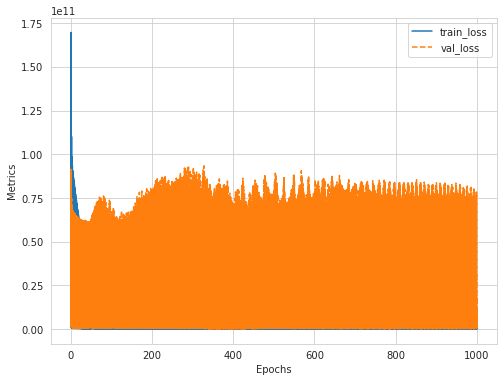
\includegraphics[width=5cm]{all_full_epoch_1000_fold_4}}
	\caption{Training \& validation loss of basic model for predicting prices}
	\label{all_full_epoch_1000}
\end{figure*}

\begin{table}[!htbp]
	\centering
	\caption{ True and predicted prices for basic model}
	\label{basic_model_prediction_price}
	\begin{tabular}{| c | c | c |}
		\hline
		Predictions & Actual Price & Price Error \% \\
		\hline
		0 & 695 & 100 \\
		\hline
		593571 & 350000 & 69.59 \\
		\hline
		177140 & 130000 & 36.26 \\
		\hline
		0 & 475 & 100 \\
		\hline
		156217 & 105000 & 48.77 \\
		\hline
		509198 & 450000 & 13.15 \\
		\hline
		0 & 460 & 100 \\ 
		\hline
		389259 & 325000 & 19.77 \\
		\hline
		571157 & 585000 & 2.36 \\
		\hline
		0 & 900 & 100 \\
		\hline
	\end{tabular}
\end{table}

 It is evident from table \ref{basic_model_prediction_price} that the rental prices which are around few hundreds are all predicted to be zero, whereas the error for some sale prices can be acceptable. This could be caused by the imbalanced dataset, which contains twice as many sale data as rental data. Therefore, the weighted random sampler (WRS), which can ensure that the number of distinct classes in a mini-batch are approximately the same, is utilized to address the issue .
 \\
 
Figure \ref{all_full_epoch_1000_ws} illustrates the training \& validation losses after applying WRS. Base on these figures, the model trained in fold two is selected for the evaluation, and the first ten predicted prices are displayed in table \ref{basic_model_prediction_price_ws}. The metrics of this model are $MSE = 4635616774$, and $R^2 = 0.86$. 

\begin{figure*}[!htbp]
	\centering
	\subfigure[Fold 0]{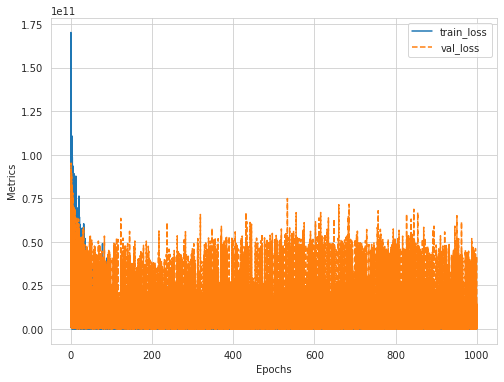
\includegraphics[width=5cm]{all_weighted_sampler_full_epoch_1000_fold_0}}
	\hfill
	\subfigure[Fold 1]{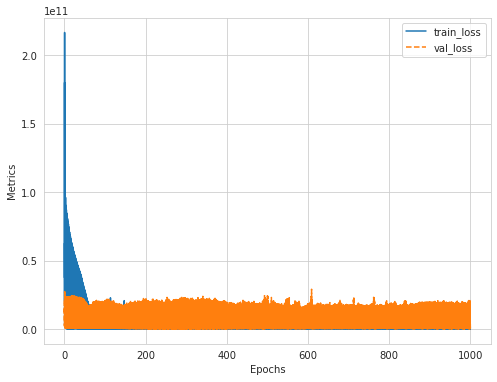
\includegraphics[width=5cm]{all_weighted_sampler_full_epoch_1000_fold_1}}
	\hfill
	\subfigure[Fold 2]{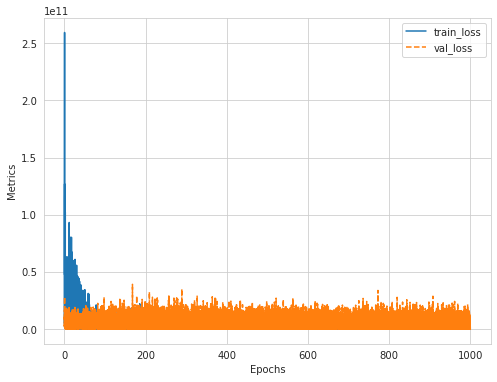
\includegraphics[width=5cm]{all_weighted_sampler_full_epoch_1000_fold_2}}
	\hfil
	\subfigure[Fold 3]{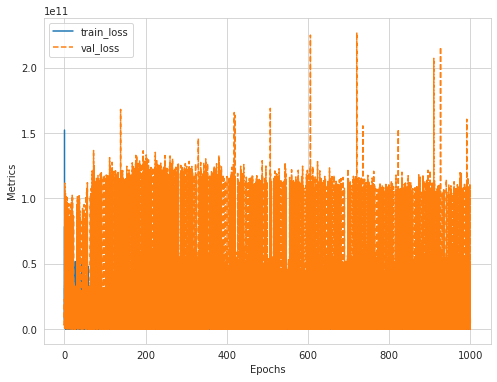
\includegraphics[width=5cm]{all_weighted_sampler_full_epoch_1000_fold_3}}
	\hfil
	\subfigure[Fold 4]{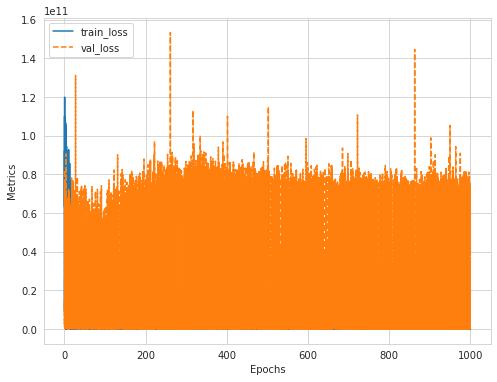
\includegraphics[width=5cm]{all_weighted_sampler_full_epoch_1000_fold_4}}
	\caption{Training \& validation loss for basic model (WRS applied)}
	\label{all_full_epoch_1000_ws}
\end{figure*}

\begin{table}[!htbp]
	\centering
	\caption{True \& predicted prices for basic model (WRS applied)}
	\label{basic_model_prediction_price_ws}
	\begin{tabular}{| c | c | c |}
		\hline
		Prediction & True Price & Error \% \\
		\hline
		764 & 695 & 10.06 \\
		\hline
		0 & 1 & 100 \\
		\hline
		233418 & 130000 & 79.55 \\
		\hline
		619 & 475 & 30.37 \\
		\hline
		91812 & 105000 & 12.55 \\
		\hline
		575859 & 450000 & 27.96 \\
		\hline
		595 & 460 & 29.38 \\ 
		\hline
		360867 & 325000 & 11.03 \\
		\hline
		655685 & 585000 & 12.08 \\
		\hline
		1149 & 900 & 27.66 \\
		\hline
	\end{tabular}
\end{table}

The predicted rental prices in table \ref{basic_model_prediction_price_ws} are not zero, but it should be noted that one of the actual prices is an outlier which has the potential to impact the performance significantly. Therefore, all the outliers (actual prices less than 100) are removed from the dataset, and the model is retrained.
\\

Figure \ref{all_full_epoch_1000_outlier_removed} depicts the training and validation losses after removing the outliers, and the model trained on fold one is chosen for evaluation based on its performance. Some actual and predicted prices are displayed in table \ref{basic_model_prediction_price_outlier_removed}. This model has following metrics, $MSE = 4580892828$, and $R^2 = 0.87$. 
\begin{figure*}[!htbp]
	\centering
	\subfigure[Fold 0]{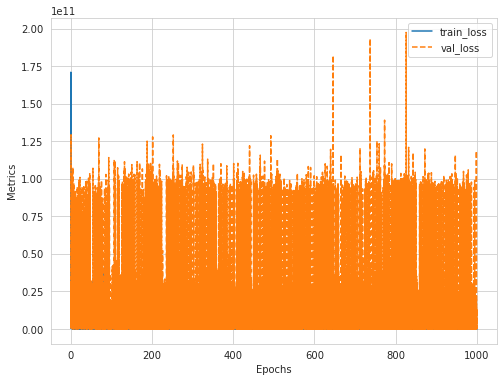
\includegraphics[width=5cm]{all_removed_weighted_sampler_full_epoch_1000_fold_0}}
	\hfill
	\subfigure[Fold 1]{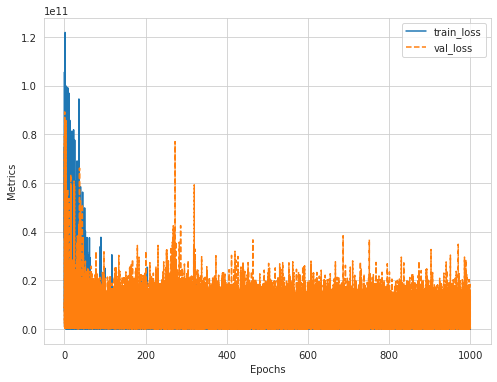
\includegraphics[width=5cm]{all_removed_weighted_sampler_full_epoch_1000_fold_1}}
	\hfill
	\subfigure[Fold 2]{\includegraphics[width=5cm]{all_removed_weighted_sampler_full_epoch_1000_fold_2}}
	\hfil
	\subfigure[Fold 3]{\includegraphics[width=5cm]{all_removed_weighted_sampler_full_epoch_1000_fold_3}}
	\hfil
	\subfigure[Fold 4]{\includegraphics[width=5cm]{all_removed_weighted_sampler_full_epoch_1000_fold_4}}
	\caption{Training \& validation loss for basic model (outliers removed)}
	\label{all_full_epoch_1000_outlier_removed}
\end{figure*}

\begin{table}[!htbp]
	\centering
	\caption{True \& predicted prices for basic model (outlier removed)}
	\label{basic_model_prediction_price_outlier_removed}
	\begin{tabular}{| c | c | c |}
		\hline
		Predicted Price & Actual Price & Error \% \\
		\hline
		92743 & 105000 & 11.67 \\
		\hline
		527 & 475 & 10.96 \\
		\hline
		183196 & 180000 & 1.77\\
		\hline
		802 & 1250 & 35.77 \\
		\hline
		522 & 395 & 32.27 \\
		\hline
		159249 & 230000 & 30.76 \\
		\hline
		1119 & 950 & 17.88 \\ 
		\hline
		74438 & 60000 & 24.06 \\
		\hline
		345296 & 285000 & 21.15 \\
		\hline
		115000 & 127500 & 9.80 \\
		\hline
	\end{tabular}
\end{table}

\subsection{Complex Model: Predicting Prices}
\label{complex_price}
The training and validation losses of this model are depicted in figure \ref{all_complex_full_epoch_1000}. The predictions made by the model in fold two are displayed in table \ref{complex_model_prediction_price}, along with its metrics, $MSE = 70788722849$, and $R^2 = -1.11$. Clearly, the complex model is not learning, and this might be caused by error hyperparameters. Therefore, the model is tuned so that its performance could be improved. 
\\
\begin{figure*}[!htbp]
	\centering
	\subfigure[Fold 0]{\includegraphics[width=5cm]{all_complex_full_epoch_1000_fold_0}}
	\hfill
	\subfigure[Fold 1]{\includegraphics[width=5cm]{all_complex_full_epoch_1000_fold_1}}
	\hfill
	\subfigure[Fold 2]{\includegraphics[width=5cm]{all_complex_full_epoch_1000_fold_2}}
	\hfil
	\subfigure[Fold 3]{\includegraphics[width=5cm]{all_complex_full_epoch_1000_fold_3}}
	\hfil
	\subfigure[Fold 4]{\includegraphics[width=5cm]{all_complex_full_epoch_1000_fold_4}}
	\caption{Training \& validation loss (Model for predicting prices)}
	\label{all_complex_full_epoch_1000}
\end{figure*}

\begin{table}[!htbp]
	\centering
	\caption{ True and predicted prices for basic model}
	\label{complex_model_prediction_price}
	\begin{tabular}{| c | c | c |}
		\hline
		Predictions & True Price & Error \% \\
		\hline
		0 & 1300 & 100 \\
		\hline
		0 & 425000 & 100 \\
		\hline
		0 & 800000 & 100 \\
		\hline
		0 & 265000 & 100 \\
		\hline
		0 & 140000 & 100 \\
		\hline
		0 & 525 & 100 \\
		\hline
		0 & 460 & 100 \\ 
		\hline
		0 & 650000 & 100 \\
		\hline
		0 & 200000 & 100 \\
		\hline
		0 & 650 & 100 \\
		\hline
	\end{tabular}
\end{table}

Several hyperparameters, including the number of epochs, learning rate, number of neurons in each layer, and activate functions, are tuned sequentially to enhance the performance, and the result is depicted in \ref{tune}. Therefore, the complex model is trained by 300 epochs, the learning rate is 0.0001, the activate function is ReLU, and each layer consists of 256 neurons. The metrics of this model are as follows, $MSE = 4754801560$, and $R^2 = 0.85$

\begin{figure*}[!htbp]
	\centering
	\subfigure[Epochs]{\includegraphics[width=5cm]{tune_epoch} \label{tune_epoch}}
	\hfil
	\subfigure[Learning Rate]{\includegraphics[width=5cm]{tune_lr} \label{tune_lr}}
	\subfigure[Number of neurons]{\includegraphics[width=5cm]{tune_neurons} \label{tune_neurons}}
	\hfil
	\subfigure[Activate Functions]{\includegraphics[width=5cm]{tune_activate} \label{tune_activate}}
	\caption{Result of tuning hyperparameters}
	\label{tune}
\end{figure*}

\subsection{Residual Network: Predicting Prices}
Figure \ref{all_resnet_full_epoch_1000} illustrates the training and validation losses for residual networks, and the model from fold one is selected for evaluation due to its low loss. Some predicted prices are displayed in table \ref{resnet_prediction_price}; its metrics are $MSE = 4515004136$, and $R^2 = 0.86$. 
\begin{figure*}[!htbp]
	\centering
	\subfigure[Fold 0]{\includegraphics[width=5cm]{all_resnet_full_epoch_1000_fold_0}}
	\hfill
	\subfigure[Fold 1]{\includegraphics[width=5cm]{all_resnet_full_epoch_1000_fold_1}}
	\hfill
	\subfigure[Fold 2]{\includegraphics[width=5cm]{all_resnet_full_epoch_1000_fold_2}}
	\hfil
	\subfigure[Fold 3]{\includegraphics[width=5cm]{all_resnet_full_epoch_1000_fold_3}}
	\hfil
	\subfigure[Fold 4]{\includegraphics[width=5cm]{all_resnet_full_epoch_1000_fold_4}}
	\caption{Training \& validation loss (Model for predicting prices)}
	\label{all_resnet_full_epoch_1000}
\end{figure*}

\begin{table}[!htbp]
	\centering
	\caption{ True and predicted prices for basic model}
	\label{resnet_prediction_price}
	\begin{tabular}{| c | c | c |}
		\hline
		Predictions & Actual Price & Error \% \\
		\hline
		146653 & 200000 & 26.67 \\
		\hline
		434 & 475 & 8.44 \\
		\hline
		117730 & 105000 & 12.12 \\
		\hline
		1840 & 1250 & 47.26 \\
		\hline
		177246 & 180000 & 1.52 \\
		\hline
		123018 & 140000 & 12.12 \\
		\hline
		325667 & 300000 & 8.55 \\ 
		\hline
		122508 & 150000 & 18.32 \\
		\hline
		747 & 525 & 42.38 \\
		\hline
		255869 & 200000 & 27.93 \\
		\hline
	\end{tabular}
\end{table}

\subsection{Comparing models for predicting prices}
Table \ref{metrics_basic_model} summarizes the metrics of all the models for predicting prices. It is evident that the linear regression model has the worst performance since its simple architecture is incapable of extracting insight from datasets. For the basic models, their performance becomes better when WRS is applied and outliers are removed. Moreover, although the remaining two complex models have more layers and neurons, they cannot improve the accuracy significantly. Therefore, the basic model should be chosen for predicting prices because of its acceptable performance and simple architecture, which results in smaller model size and less prediction time. 
\begin{table}[!htbp]
	\centering
	\caption{Metrics of various models for predicting prices}
	\label{metrics_basic_model}
	\begin{tabular}{| l | c | c |}
		\hline
		& MSE & $R^2$ \\
		\hline
		Linear Regression Model & 66601086343 & -0.91 \\
		\hline
		Basic Model (Price and Status) & 7559964776 & 0.54 \\
		\hline
		Basic Model (Price only) & 4918700785 & 0.85 \\
		\hline
		Basic Model (WRS applied) & 4635616774 & 0.86 \\
		\hline
		Basic Model (Outliers removed) & 4580892828 & 0.87 \\
		\hline
		Complex Model & 4754801560 & 0.85 \\
		\hline
		Residual Network & 4515004136 & 0.86 \\
		\hline
	\end{tabular}
\end{table}

\subsection{Linear Regression: Predict Status of Transactions}
\label{linear_regression_status}
\subsubsection{Actual and Predicted Prices Included}
The training and validation losses of the model are depicted in figure \ref{linear_regression_status_include_full}, and all the models can converge and the losses of the last three models are comparable. Therefore, they are utilized for evaluation, and the threshold for converting numerical values into status is set to 0.5. Figure \ref{cm_included} displays the confusion matrics of three models, and their metrics are listed in table \ref{metrics_linear_regression_status_included}.
\\

From table \ref{metrics_linear_regression_status_included}, the recall has the highest values, indicating that the model can predict the completed transactions with greater confidence. However, the precision and F1 score are around 0.3, which means that the performance of these models is unacceptable. 
\begin{figure*}[!htbp]
	\centering
	\subfigure[Fold 0]{\includegraphics[width=5cm]{linear_regression_status_include_full_fold_0}}
	\hfill
	\subfigure[Fold 1]{\includegraphics[width=5cm]{linear_regression_status_include_full_fold_1}}
	\hfill
	\subfigure[Fold 2]{\includegraphics[width=5cm]{linear_regression_status_include_full_fold_2}}
	\hfil
	\subfigure[Fold 3]{\includegraphics[width=5cm]{linear_regression_status_include_full_fold_3}}
	\hfil
	\subfigure[Fold 4]{\includegraphics[width=5cm]{linear_regression_status_include_full_fold_4}}
	\caption{Training \& validation loss for linear regression model (prices included)}
	\label{linear_regression_status_include_full}
\end{figure*}

\begin{figure*}[!htbp]
	\centering
	\subfigure[Fold 2]{\includegraphics[width=5cm]{cm_included_2}}
	\hfill
	\subfigure[Fold 3]{\includegraphics[width=5cm]{cm_included_3}}
	\hfill
	\subfigure[Fold 4]{\includegraphics[width=5cm]{cm_included_4}}
	\caption{Confusion matrices for linear regression models (prices included)}
	\label{cm_included}
\end{figure*}

\begin{table}[!htbp]
	\centering
	\caption{Metrics of linear regression models (prices included)}
	\label{metrics_linear_regression_status_included}
	\begin{tabular}{| c | c | c | c | c |}
		\hline
		Fold & Accuracy & Precision & Recall & F1 Score \\
		\hline
		2 & 0.405 & 0.242 & 0.683 & 0.357 \\
		\hline
		3 & 0.423 & 0.235 & 0.747 & 0.358 \\
		\hline
		4 & 0.453 & 0.352 & 0.697 & 0.468 \\
		\hline
	\end{tabular}
\end{table}

\subsubsection{Actual and Predicted Prices Excluded}
Figure \ref{linear_regression_status_exclude_full} illustrates the training and validation losses of the models that are trained without prices. It is evident that all the models can converge, and the models from folds zero, two and four are utilized for evaluation since they have superior performance. The confusion matrices and metrics are illustrated in figure \ref{cm_excluded} and table \ref{metrics_linear_regression_status_excluded}, respectively. 
\\

In table \ref{metrics_linear_regression_status_excluded}, the recall is the highest, while the precision and F1 score are low, suggesting that although the loss can converge, the performance of models is unreliable.  Moreover, there are approximately 300 completed and 600 incompleted transactions in the testing dataset; the accuracy of the model should be 66.6\% even if it only outputs incompleted, whereas none of the linear regression models can exceed this threshold. Therefore, more complex neural networks are required for robust performance. 
\\

\begin{figure*}[!htbp]
	\centering
	\subfigure[Fold 0]{\includegraphics[width=5cm]{linear_regression_status_exclude_full_fold_0}}
	\hfill
	\subfigure[Fold 1]{\includegraphics[width=5cm]{linear_regression_status_exclude_full_fold_1}}
	\hfill
	\subfigure[Fold 2]{\includegraphics[width=5cm]{linear_regression_status_exclude_full_fold_2}}
	\hfil
	\subfigure[Fold 3]{\includegraphics[width=5cm]{linear_regression_status_exclude_full_fold_3}}
	\hfil
	\subfigure[Fold 4]{\includegraphics[width=5cm]{linear_regression_status_exclude_full_fold_4}}
	\caption{Training \& validation loss of model for status (without prices)}
	\label{linear_regression_status_exclude_full}
\end{figure*}

\begin{figure*}[!htbp]
	\centering
	\subfigure[Fold 0]{\includegraphics[width=5cm]{cm_excluded_0}}
	\hfill
	\subfigure[Fold 2]{\includegraphics[width=5cm]{cm_excluded_2}}
	\hfill
	\subfigure[Fold 4]{\includegraphics[width=5cm]{cm_excluded_4}}
	\caption{Confusion matrices for linear regression models (prices excluded)}
	\label{cm_excluded}
\end{figure*}

\begin{table}[!htbp]
	\centering
	\caption{Metrics of linear regression models (prices excluded)}
	\label{metrics_linear_regression_status_excluded}
	\begin{tabular}{| c | c | c | c | c |}
		\hline
		Fold & Accuracy & Precision & Recall & F1 Score \\
		\hline
		0 & 0.381 & 0.154 & 0.719 & 0.254 \\
		\hline
		2 & 0.514 & 0.469 & 0.722 & 0.569 \\
		\hline
		4 & 0.388 & 0.191 & 0.690 & 0.300 \\
		\hline
	\end{tabular}
\end{table}

\subsection{Transfer-baesd Model: Predict Status}
Figure \ref{transfer_based_status} illustrates the training and validation losses. The model in fold three is selected for the evaluation, and predictions are \textit{completed} regardless of the actual status. This error may be caused by the imbalanced dataset since there are 3088 complete transactions, whereas more than twice as many incomplete transactions. 

\begin{figure*}[!htbp]
	\centering
	\subfigure[Fold 0]{\includegraphics[width=5cm]{status_removed_full_epoch_1000_fold_0}}
	\hfill
	\subfigure[Fold 1]{\includegraphics[width=5cm]{status_removed_full_epoch_1000_fold_1}}
	\hfill
	\subfigure[Fold 2]{\includegraphics[width=5cm]{status_removed_full_epoch_1000_fold_2}}
	\hfil
	\subfigure[Fold 3]{\includegraphics[width=5cm]{status_removed_full_epoch_1000_fold_3}}
	\hfil
	\subfigure[Fold 4]{\includegraphics[width=5cm]{status_removed_full_epoch_1000_fold_4}}
	\caption{Training \& validation loss of transfer-based model}
	\label{transfer_based_status}
\end{figure*}

Therefore, WRS is applied to ensure that the data in each mini-batch is balanced, and the results are depicted in figure \ref{transfer_based_status_WRS}. The model's output is 0.499189 for all the inputs, which is incorrect. 
\\

The architecture of this model may be responsible for these outcomes. A pre-trained model for predicting prices is loaded whose outputs range from several hundred to several thousand. However, the other inputs are normalized, meaning that they range from -1 to 1. Therefore, the inputs are on significantly different scales, resulting in the model focusing on the feature with a larger magnitude, prices in this case, while ignoring other features. 
\\

\begin{figure*}[!htbp]
	\centering
	\subfigure[Fold 0]{\includegraphics[width=5cm]{status_ws_removed_full_epoch_1000_fold_0}}
	\hfill
	\subfigure[Fold 1]{\includegraphics[width=5cm]{status_ws_removed_full_epoch_1000_fold_1}}
	\hfill
	\subfigure[Fold 2]{\includegraphics[width=5cm]{status_ws_removed_full_epoch_1000_fold_2}}
	\hfil
	\subfigure[Fold 3]{\includegraphics[width=5cm]{status_ws_removed_full_epoch_1000_fold_3}}
	\hfil
	\subfigure[Fold 4]{\includegraphics[width=5cm]{status_ws_removed_full_epoch_1000_fold_4}}
	\caption{Training \& validation loss of transfer-based model (WRS applied)}
	\label{transfer_based_status_WRS}
\end{figure*}

In order to address this issue, the layout of the model is preserved, but the parameters of the pre-trained model are not frozen. This is because despite the model output being on a different scale, its previous performance demonstrated that this architecture is capable of predicting prices with acceptable error rates. Therefore, it is anticipated that removing parameters while retaining architecture would output the prices on the same scale as other features, thereby facilitating the output of the entire model. 
\\

Figure \ref{transfer_based_status_no_freeze} displays the training and validation losses for the latest modlfication. The models from folds two and four have the best performance and are used for evaluation. The results for the two models are comparable, both of them output the same value, which is approximately 0.5, regardless of the actual status. These incorrect results indicate that the transfer-based model cannot predict the status of transactions.  

\begin{figure*}[!htbp]
	\centering
	\subfigure[Fold 0]{\includegraphics[width=5cm]{status_ws_removed_full_no_freeze_fold_0}}
	\hfill
	\subfigure[Fold 1]{\includegraphics[width=5cm]{status_ws_removed_full_no_freeze_fold_1}}
	\hfill
	\subfigure[Fold 2]{\includegraphics[width=5cm]{status_ws_removed_full_no_freeze_fold_2}}
	\hfil
	\subfigure[Fold 3]{\includegraphics[width=5cm]{status_ws_removed_full_no_freeze_fold_3}}
	\hfil
	\subfigure[Fold 4]{\includegraphics[width=5cm]{status_ws_removed_full_no_freeze_fold_4}}
	\caption{Training \& validation loss of transfer-based model (no frozen parameters)}
	\label{transfer_based_status_no_freeze}
\end{figure*}

\subsection{Basic Model: Price Included}
\label{basic_status_training_included}
The training and validation losses are displayed in figure \ref{basic_status}. Even though all the losses can converge from these graphs, the models would only output a value of approximately 0.5 regardless of the actual status.
\\

\begin{figure*}[!htbp]
	\centering
	\subfigure[Fold 0]{\includegraphics[width=5cm]{status_basic_no_bs_dropout_0}}
	\hfill
	\subfigure[Fold 1]{\includegraphics[width=5cm]{status_basic_no_bs_dropout_1}}
	\hfill
	\subfigure[Fold 2]{\includegraphics[width=5cm]{status_basic_no_bs_dropout_2}}
	\hfil
	\subfigure[Fold 3]{\includegraphics[width=5cm]{status_basic_no_bs_dropout_3}}
	\hfil
	\subfigure[Fold 4]{\includegraphics[width=5cm]{status_basic_no_bs_dropout_4}}
	\caption{Training \& validation loss of basic model for predicting status (with prices)}
	\label{basic_status}
\end{figure*}

In order to evaluate the cause of this error, outputs from the hidden layers are obtained, with the result that all the hidden layer outputs are zero indicating that hidden layers and inputs have no effect, resulting in the model outputs being 0.5. To further analyze this error, the outputs of the activation functions are acquired, and they are illustrated in figure \ref{vanish_gradient}. It is evident that the outputs decreae as the depth increases, and in some folds, they even become approximately zero.
\\

\begin{figure*}[!htbp]
	\centering
	\subfigure[Fold 0]{\includegraphics[width=5cm]{vanish0}}
	\hfill
	\subfigure[Fold 1]{\includegraphics[width=5cm]{vanish1}}
	\hfill
	\subfigure[Fold 2]{\includegraphics[width=5cm]{vanish2}}
	\hfil
	\subfigure[Fold 3]{\includegraphics[width=5cm]{vanish3}}
	\hfil
	\subfigure[Fold 4]{\includegraphics[width=5cm]{vanish4}}
	\caption{The outputs of activation functions}
	\label{vanish_gradient}
\end{figure*}

The problem causing the models to output 0.5 is the vanishing gradient which is mitigated by two solutions. The first method is the initialization scheme; the Keiming initialization scheme is used since the activation functions are ReLU in this model. The second approach is inserting batch normalization (BN) between linear layers and activation functions. 
\\

The results of configuring the initialization scheme and inserting BN are displayed in figure \ref{status_overfitting}. The models are overfitting since the validation losses continue to increase while the training losses remain constant. Therefore, regularization should be applied so that overfitting can be prevented. In this project, dropout, a type of regularization that can avoid the neural network relying on a single neuron, is inserted into the model between BN and activation functions at a ratio of 0.5. 
\\

Figure \ref{status_dropout} demonstrates the effect of applying dropout. The overfitting is avoided, but the losses oscillate around 0.7 with neither decreasing nor increasing trend. Despite these defects, the models have the lowest losses for predicting status. Therefore, they are evaluated. The model from the second fold is chosen for evaluation because it has the lowest loss and oscillation range based on these loss plots. The confusion matrix are depicted in figure \ref{status_dropout_prediction}, and its metrics are as follows, $accuracy = 0.7188$, $precision = 0.8113$, $recall = 0.7845$ and $F1 score = 0.7977$.
\\

\begin{figure*}[!htbp]
	\centering
	\subfigure[Fold 0]{\includegraphics[width=5cm]{status_overfitting0}}
	\hfill
	\subfigure[Fold 1]{\includegraphics[width=5cm]{status_overfitting1}}
	\hfill
	\subfigure[Fold 2]{\includegraphics[width=5cm]{status_overfitting2}}
	\hfil
	\subfigure[Fold 3]{\includegraphics[width=5cm]{status_overfitting3}}
	\hfil
	\subfigure[Fold 4]{\includegraphics[width=5cm]{status_overfitting4}}
	\caption{Training \& validation losses (initialization scheme and BN)}
	\label{status_overfitting}
\end{figure*}

\begin{figure*}[!htbp]
	\centering
	\subfigure[Fold 0]{\includegraphics[width=5cm]{status_append_ws_removed_full_no_freeze_fold_0}}
	\hfill
	\subfigure[Fold 1]{\includegraphics[width=5cm]{status_append_ws_removed_full_no_freeze_fold_1}}
	\hfill
	\subfigure[Fold 2]{\includegraphics[width=5cm]{status_append_ws_removed_full_no_freeze_fold_2}}
	\hfil
	\subfigure[Fold 3]{\includegraphics[width=5cm]{status_append_ws_removed_full_no_freeze_fold_3}}
	\hfil
	\subfigure[Fold 4]{\includegraphics[width=5cm]{status_append_ws_removed_full_no_freeze_fold_4}}
	\caption{Training \& validation losses (dropout inserted)}
	\label{status_dropout}
\end{figure*}

\begin{figure}[!htbp]
	\centering
	\includegraphics[width=10cm]{cm_dropout2}
	\caption{The confusion matrix of the model from fold two}
	\label{status_dropout_prediction}
\end{figure}

From the confusion matrix, the model can predict the class of \textit{Not Complete} with more than 80\% accuracy, whereas the forecast of the other class is approximately 50\%, which is not acceptable. Therefore, the model's performance must be improved by tuning some hyperparameters such as the learning rate and dropout ratio. Figure \ref{status_tuned} illustrates the losses after tuning hyperparameters, and it can be seen that all the losses initially decrease and then oscillate. 
\\

\begin{figure*}[!htbp]
	\centering
	\subfigure[Fold 0]{\includegraphics[width=5cm]{status_v3_fold_0}}
	\hfill
	\subfigure[Fold 1]{\includegraphics[width=5cm]{status_v3_fold_1}}
	\hfill
	\subfigure[Fold 2]{\includegraphics[width=5cm]{status_v3_fold_2}}
	\hfil
	\subfigure[Fold 3]{\includegraphics[width=5cm]{status_v3_fold_3}}
	\hfil
	\subfigure[Fold 4]{\includegraphics[width=5cm]{status_v3_fold_4}}
	\caption{Training \& validation losses (hyperparameters tuned)}
	\label{status_tuned}
\end{figure*}

The model in fold three is selected due to ist low loss and narrow oscillation. The confusion matrix is displayed in figure \ref{status_tuned_prediction}, and its metrics are $accuracy = 0.8177$, $recall = 0.8350$, $precision = 0.9138$ and $F1 score = 0.8726$. It is evident that the overall accuracy has enhanced and the prediction of \textit{Not Completed} exceeds 90\%, while it is around 60\% for \textit{Completed} transactions. Moreover, the models become overfitting as the oscillation range expands in figure \ref{status_tuned}. Therefore, the model is retrained with fewer epochs and higher ratio of dropout. 
\\

\begin{figure}[!htbp]
	\centering
	\includegraphics[width=10cm]{cm_tuned}
	\caption{The confusion matrix of the model after tuning hyperparameters}
	\label{status_tuned_prediction}
\end{figure}

Figure \ref{status_fewer} depicts the training and validation losses, where the trends initially decrease and oscillate around 0.5, and the models are less overfitting since the oscillation ranges are constant. The model in fold three is selected for evaluation, and figure \ref{status_fewer_prediction} illustrates the confusion matrix, along with the following metrics: $accuracy = 0.8355$, $recall = 0.8293$, $precision = 0.9560$, and $F1 score = 0.8882$. 
\\

\begin{figure*}[!htbp]
	\centering
	\subfigure[Fold 0]{\includegraphics[width=5cm]{status_v4_fold_0}}
	\hfill
	\subfigure[Fold 1]{\includegraphics[width=5cm]{status_v4_fold_1}}
	\hfill
	\subfigure[Fold 2]{\includegraphics[width=5cm]{status_v4_fold_2}}
	\hfil
	\subfigure[Fold 3]{\includegraphics[width=5cm]{status_v4_fold_3}}
	\hfil
	\subfigure[Fold 4]{\includegraphics[width=5cm]{status_v4_fold_4}}
	\caption{Training \& validation losses (fewer epoch and adjusted dropout)}
	\label{status_fewer}
\end{figure*}

\begin{figure}[!htbp]
	\centering
	\includegraphics[width=9cm]{cm_fewer}
	\caption{The confusion matrix of the model (fewer epochs and adjusted dropout)}
	\label{status_fewer_prediction}
\end{figure}

From the evaluation results, it is obvious that the overall performance has enhanced, but the issue of predicting the completed transactions still exists. The imbalanced dataset could be the cause of this problem. Although the WRS is applied during training, resulting in the balanced mini-batches, the \textit{Completed} class is the minority and is therefore insufficient for the model to extract its patterns. Consequently, a bias is considered to modify the sampling weight so that the number of completed transactions can be increased in each mini-batch which is anticipated to improve the accuracy of predictions. The attempted biases are 0.05, 0.1 and 0.15, with the corresponding losses shown in figures \ref{status_005}, \ref{status_01}, and \ref{status_015}. 
\\

\begin{figure*}[!htbp]
	\centering
	\subfigure[Fold 0]{\includegraphics[width=5cm]{status_bias_005_fold_0}}
	\hfill
	\subfigure[Fold 1]{\includegraphics[width=5cm]{status_bias_005_fold_1}}
	\hfill
	\subfigure[Fold 2]{\includegraphics[width=5cm]{status_bias_005_fold_2}}
	\hfil
	\subfigure[Fold 3]{\includegraphics[width=5cm]{status_bias_005_fold_3}}
	\hfil
	\subfigure[Fold 4]{\includegraphics[width=5cm]{status_bias_005_fold_4}}
	\caption{Training \& validation losses (prices included and bias = 0.05)}
	\label{status_005}
\end{figure*}

\begin{figure*}[!htbp]
	\centering
	\subfigure[Fold 0]{\includegraphics[width=5cm]{status_bias_01_fold_0}}
	\hfill
	\subfigure[Fold 1]{\includegraphics[width=5cm]{status_bias_01_fold_1}}
	\hfill
	\subfigure[Fold 2]{\includegraphics[width=5cm]{status_bias_01_fold_2}}
	\hfil
	\subfigure[Fold 3]{\includegraphics[width=5cm]{status_bias_01_fold_3}}
	\hfil
	\subfigure[Fold 4]{\includegraphics[width=5cm]{status_bias_01_fold_4}}
	\caption{Training \& validation losses (prices included and bias = 0.1)}
	\label{status_01}
\end{figure*}

\begin{figure*}[!htbp]
	\centering
	\subfigure[Fold 0]{\includegraphics[width=5cm]{status_bias_015_fold_0}}
	\hfill
	\subfigure[Fold 1]{\includegraphics[width=5cm]{status_bias_015_fold_1}}
	\hfill
	\subfigure[Fold 2]{\includegraphics[width=5cm]{status_bias_015_fold_2}}
	\hfil
	\subfigure[Fold 3]{\includegraphics[width=5cm]{status_bias_015_fold_3}}
	\hfil
	\subfigure[Fold 4]{\includegraphics[width=5cm]{status_bias_015_fold_4}}
	\caption{Training \& validation losses (prices included and bias = 0.15)}
	\label{status_015}
\end{figure*}

Folds three, two, and four are selected for evaluation when bias is 0.05, 0.1, and 0.15, respectively. Figure \ref{status_bias_cm} and table \ref{status_bias_metrics} depicts their confusion matrices and metrics along with the model that bias is not applied. The accuracy for predicting the \textit{Completed} class improves with the bias increases, which is the same as the expectation. However, as a trade-off, the precision in table \ref{status_bias_metrics} is decreasing, indicating that the correctness of predicting the other class decreases, resulting in the decline of the overall performance.

\begin{figure*}[!htbp]
	\centering
	\subfigure[bias = 0]{\includegraphics[width = 7.5cm]{cm_fewer}}
	\hfil
	\subfigure[bias = 0.05]{\includegraphics[width=7.5cm]{cm_005_fold_1}}
	\hfill
	\subfigure[bias = 0.1]{\includegraphics[width=7.5cm]{cm_01_fold_4}}
	\hfill
	\subfigure[bias = 0.15]{\includegraphics[width=7.5cm]{cm_015_fold_2}}
	\caption{Confusion matrices of models with various biases (price included)}
	\label{status_bias_cm}
\end{figure*}

\begin{table}[!htbp]
	\centering
	\caption{Metrics of models with various biases (price included)}
	\label{status_bias_metrics}
	\begin{tabular}{| c | c | c | c | c |}
		\hline
		Bias & Accuracy & Recall & Precision & F1 Score \\
		\hline
		0.00 & 0.8355 & 0.8293 & 0.9560 & 0.8882 \\
		\hline
		0.05 & 0.8177 & 0.8340 & 0.9154 & 0.8728 \\
		\hline
		0.10 & 0.8266 & 0.8614 & 0.8894 & 0.8752 \\
		\hline
		0.15 & 0.8011 & 0.8682 & 0.8357 & 0.8516 \\
		\hline
	\end{tabular}
\end{table}

Furthermore, when comparing the models with biases are 0 and 0.05, the correct prediction of the class \textit{Completed} increases from 57\% to 60\%, but the accuracy for the \textit{Not Completed} drops from 95\% to 91\%, indicating that a bias of 0.05 is not worthwhile. Using the same approach when biases are 0 and 0.15, the corrected predicted \textit{Completed} class increases by 20\%, while the precision and the overall performance decline significantly. When comparing models with biases of 0 and 0.1, the correct prediction of the \textit{Completed} transactions increases by more than 10\%, and a decrease in the overall performance and precision can be acceptable. 
\\

After tuning hyperparameters and modifying the architecture, the final layout of the basic model for predicting transaction status is demonstrated in figure \ref{basic_status_final_layout}. 

\begin{figure}[H]
	\centering
	\includegraphics[height=\textheight]{basic_status_final_layout}
	\caption{The final layout of the basic model for status (with price)}
	\label{basic_status_final_layout}
\end{figure}

\subsection{Ablation Study}
\subsubsection{Transaction Status}
Section \ref{linear_regression_status} demonstrates that the models should be trained with prices included and excluded to accurately predict the transaction status. As part of the ablation study, models without prices are trained, and other features, such as the number of various rooms, postcode are also tested so that the most significant attribute can be determined. The metrics of removing one of the features are shown in table \ref{ablation_status}.

\begin{table}[H]
	\centering
	\caption{Metrics after removing one of the input features}
	\label{ablation_status}
	\begin{tabular}{| c | c | c | c | c | }
		\hline
		Removed Feature & Accuracy & Recall & Precision & F1 Score \\
		\hline
		None & 0.8266 & 0.8614 & 0.8894 & 0.8752 \\
		\hline
		Postcode & 0.8211 & 0.8697 & 0.8682 & 0.8689 \\
		\hline
		Bedroom Number & 0.8144 & 0.8648 & 0.8634 & 0.8641 \\
		\hline
		Kitchen Number & 0.8211 & 0.8637 & 0.8764 & 0.8700 \\
		\hline
		Living Room Number & 0.8177 & 0.8596 & 0.8764 & 0.8679 \\
		\hline
		Bathroom Number & 0.8244 & 0.8667 & 0.8780 & 0.8723 \\
		\hline
		Dining Room Number & 0.8155 & 0.8615 & 0.8699 & 0.8656 \\
		\hline
		Other Room Number & 0.8055 & 0.8630 & 0.8504 & 0.8566 \\
		\hline
		Predicted Price & 0.8044 & 0.8616 & 0.8504 & 0.8559 \\
	\end{tabular}
\end{table}

\subsubsection{Property Prices}

%%%%%%%%%%%%%%%%%%%%%%%%%%%%%%%%%%%%
\chapter{Conclusion and Future Work}
\section{Future Work}
\subsection{Dataset}
This project aims to develop a model to predict if a property can be sold across the UK. The distribution of the properties used for training is shown in figure \ref{uk_distribution}. A significant number of properties are located in England, and the data outside of England are located in Cardiff, Edinburgh, Glasgow, and Aberdeen. Therefore, the result will be unreliable if a property is not located in these areas, such as Belfast. In addition, the raw dataset contains approximately 35000 records, whereas a significant number of missing values lead to the dataset for training and testing containing less than 9000 records.
\\

Moreover, only the layouts and facilities of properties are used for prediction. However, in the research conducted by \citet{RN20}, the local economic data was collected and used with property data to forecast prices. Therefore, the dataset utilized in the current project can be incorporated with economical attributes, including GDP and CPI, to obtain a more robust performance. 
\\

Furthermore, London is the largest city in the UK, with distinct infrastructure and landmarks, and there are various online dataset about London. Therefore, the properties in this area could be analyzed separately. For instance, other attributes, such as the nearest tube station and the features provided by \citet{RN26}, can be inserted into the current dataset for training the model, resulting in more accurate predictions for London. 

\begin{figure}[H]
	\centering
	\includegraphics[width=\linewidth]{uk_distribution}
	\caption{The distribution of the properties used in this project}
	\label{uk_distribution}
\end{figure}

\subsection{Training the Models}
The hyperparameters were tuned sequentially when training the complex model for predicting prices (section \ref{complex_price}) due to the time limitation. Although this approach is unlikely to obtain the optimal combination of hyperparameters, the performance can still be improved. A similar approach for tuning employs nested loops, whereas its problem is that it requires significant time and hardware resources. Grid search is superior, which selects hyperparameters randomly and then trains the model. This method may not obtain the optimal combination of hyperparameters, but it is less expensive than the first approach \citep{RN38}. Bayesian optimization selects new hyperparameters based on the previous performance \citep{RN38}. It is regarded as the best method for tuning since the optimal combination can be obtained at the lowest cost. 

\subsection{Models}
In this project, only neural networks were developed, and their performance was comparable to those created by \citet{RN37}. However, there are other available ML algorithms. \citet{RN17} stated that the random forest has the best performance in their study, whereas \citet{RN20} argued that XGBoost is the model with the highest accuracy instead of random forest. The models utilized in their research and the models reviewed in section \ref{model_review} should be attempted so that the accuracy of predicting the property transaction can be improved. 

\section{Ethics}
EweMove provided the datasets used in this project. No humans were involved in the data preparation phase, and all the data in the datasets were anonymous and unidentifiable, meaning there were no potential privacy concerns. In addition, the General Data Protection Regulation (EU) was adhered to throughout the development of the project to prevent data abuse and leakage. 

\section{Conclusion}
This project aims to develop an ML model for predicting property transactions, and the main objective has been accomplished. The raw dataset was preprocessed by removing missing values, encoding categorical features, standardizing the data, and splitting datasets. Then, the training data was used as the input for price prediction models, which were evaluated based on multiple metrics. The result demonstrated that an accuracy of 86\% could be achieved. The model with the highest accuracy was then employed to predict prices for all the properties, which was one of the inputs to forecasting the transaction status. After training and testing the models for predicting status, the final result was that approximately 83\% of real estate transactions could be precisely predicted. 

%% bibliography
\bibliographystyle{unsrtnat}
\bibliography{proposal}

\end{document}
